\documentclass[11pt, a4paper]{article}
\usepackage[a4paper, total={6.5 in,9in}]{geometry}
\usepackage[slovene]{babel}
\usepackage[utf8]{inputenc}
\usepackage[T1]{fontenc}
\usepackage{lmodern}
\usepackage{amsmath}
\usepackage{ amssymb }
\usepackage{amsfonts}
\usepackage{amsthm}
\usepackage{comment}
\usepackage{url}
\usepackage{gensymb}
\usepackage{subcaption}
\usepackage[pdftex]{graphicx}
\usepackage[section]{placeins}
\usepackage{mathtools}
\usepackage{float}
\usepackage{epstopdf}
%\renewcommand{\vec}[1]{\mathbf{#1}}
\usepackage{hyperref}
\usepackage{wrapfig}

\pagestyle{plain}

\begin{document}

    \begin{center}
    {\LARGE\bfseries 13. Metoda maksimalne entropije in linearna napoved \par}
    \vspace{1cm}
    
    {\Large Domača naloga pri predmetu Modelska analiza I\par}
    \vspace{0.2cm}
    {\normalsize Avtor: Matic Noč \par}
    \vspace{0.2cm}    
    {\normalsize 15.1.2018\par}    

    
    \end{center}
\section{Uvod}
Pri tej nalogi smo spoznali metodo maksimalne entropije. V prvem delu naloge smo po tej metodi določili frekvenčni spekter signalov in si ogledali odvisnosti od števila polov in od gostote prikaza. Metodo smo tudi primerjali z rezultati iz prejšnje naloge, kjer smo frekven£ni spekter določili z metodo FFT. V drugem delu pa smo metodo uporabili za linearno napoved podatkov na podlagi prve polovice podatkov. 

\section{Frekvenčni spekter}
Pri prvi nalogi smo signaloma na datotekah $val2.dat$, $val3.dat$ in $co2.dat$ določili frekvenčni spekter s pomočjo metode MEM. V datoteki s koncentracijo $CO_2$ v zraku smo upoštevali splošen (linearen) letni trend in preizkusili delovanje metode v odvisnosti od števila polov in gostote prikaza. Nato smo natančnost metode primerjali še z rezultati, ki jih da FFT ob uporabi filtrov in sestavili testni signal iz vsote sinusnih členov z bližnjimi frekvencami ter raziskali ločljivost metode.\newline
Naš signal $S_n$ želimo v približku zapisati kot
\begin{equation}
\widetilde{S}_n = -\sum_{k=1}^p a_k S_{n-k} + C_n,
\end{equation}
kjer $C_n$ predstavlja odklon. Kot smo izpeljali na predavanjih lahko razliko med signalom in približkom minimiziramo pri $p$ parametrih
\begin{equation}
\epsilon = \sum_n (S_n - \widetilde{S}_n)^2,
\end{equation}
\begin{equation}
\epsilon_{min}^p = R(0) + \sum_{k=1}^p a_k R(k),
\end{equation}
kjer je 
\begin{equation}
R(k) = E[S_nS_{n+k}] = \frac{1}{N-k} \sum_{j=0}^{N-j-1} S_j S_{j+k}
\end{equation}
avtokorelacija signala $R$ in $N$ dolžina našega signala. Ko nato izračunamo vrednosti $R_k$ lahko rešimo sistem enačb $\underline{M}\vec{a} = -\vec{R}_1$, iz katerih dobimo vrednosti parametrov $a_k$ in nato pole prenosne funkcije
\begin{equation}
H(z) = \frac{1}{1+\sum_{k=1}^{p} a_k z^{-k}}.
\end{equation}
Poli prenosne funkcije $z_f$ so tako ničle imenovalca, t.j.
\begin{equation}
1+\sum_{k=1}^{p} a_k z_f^{-k},
\end{equation}
upoštevamo pa, da če ničle $z_f$ padejo izven enotskega kroga, naredimo preslikavo $z \rightarrow \frac{1}{\bar{z}}$, da jih preslikamo nazaj vanj.\newline
Frekvenčni spekter tako dobimo z 
\begin{equation}
P(\omega) = |1 + \sum_{k=1}^p a_k e^{-i\omega k }|^{-2}.
\end{equation}
\subsection{Primerjava FFT in MEM za frekvenčni spekter iz $val3.dat$ in $val2.dat$}
Najprej si poglejmo kakšne so ničle polov za različne stopnje polinoma $p$. Pri tem reskaliramo skalo $x$, da nam frekvence ustrezajo prejšni nalogi.
\newline

\begin{figure}[H]
\centering
  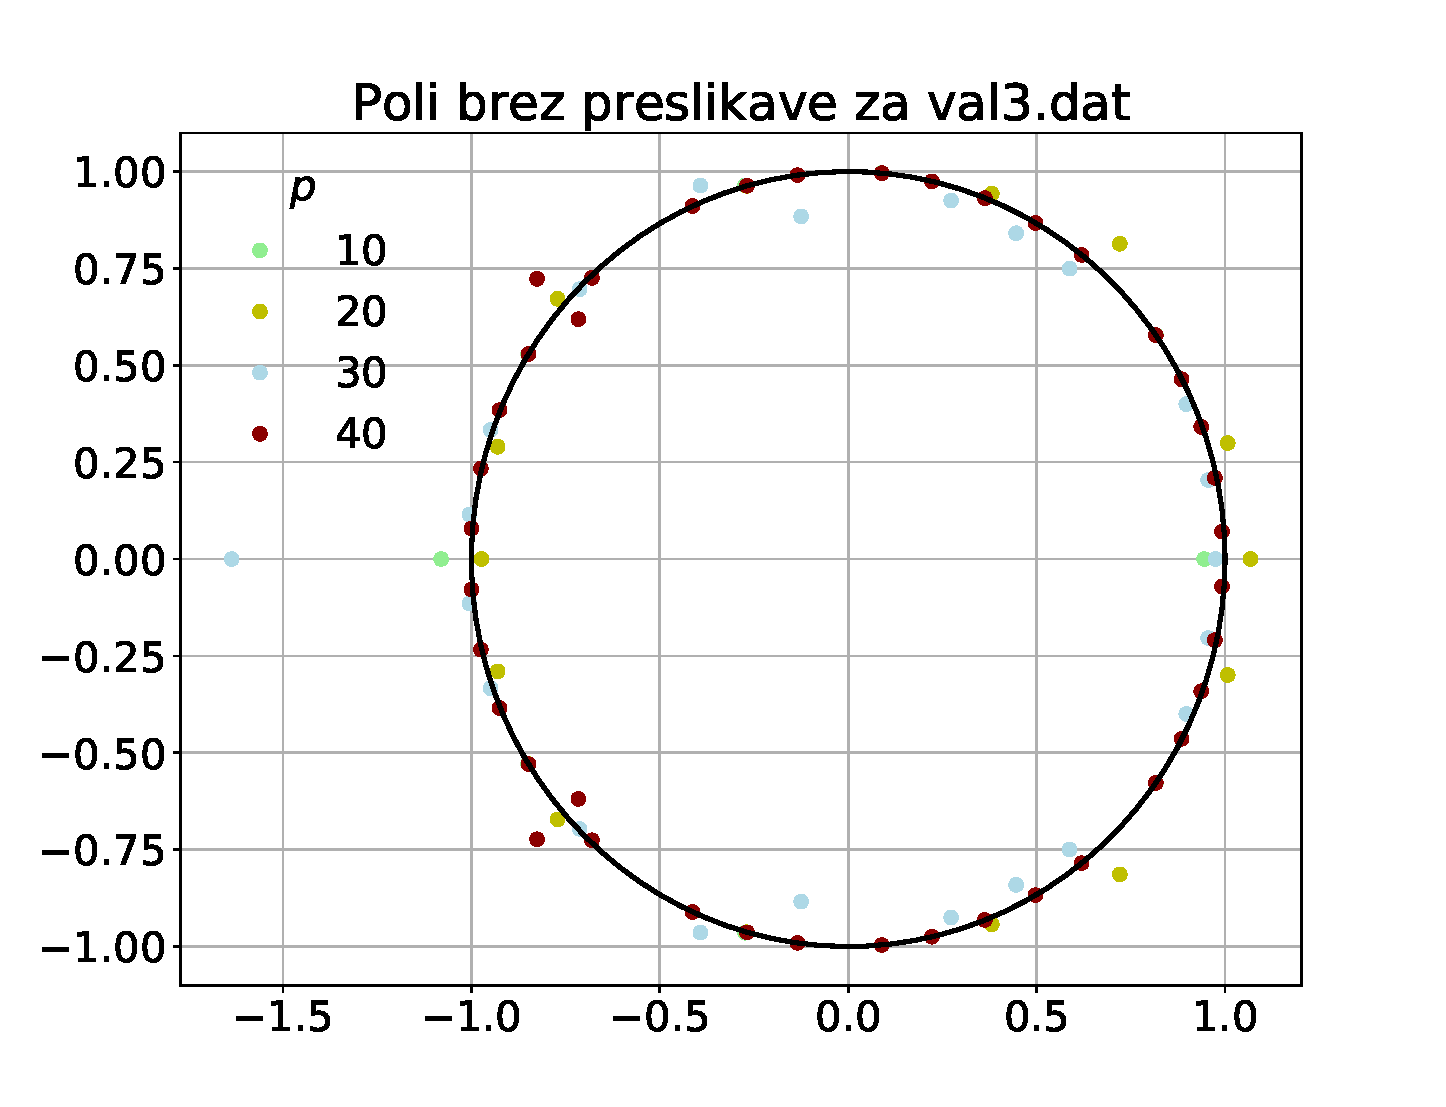
\includegraphics[width=8cm, height=5cm]{prva_primerjava1.pdf}
  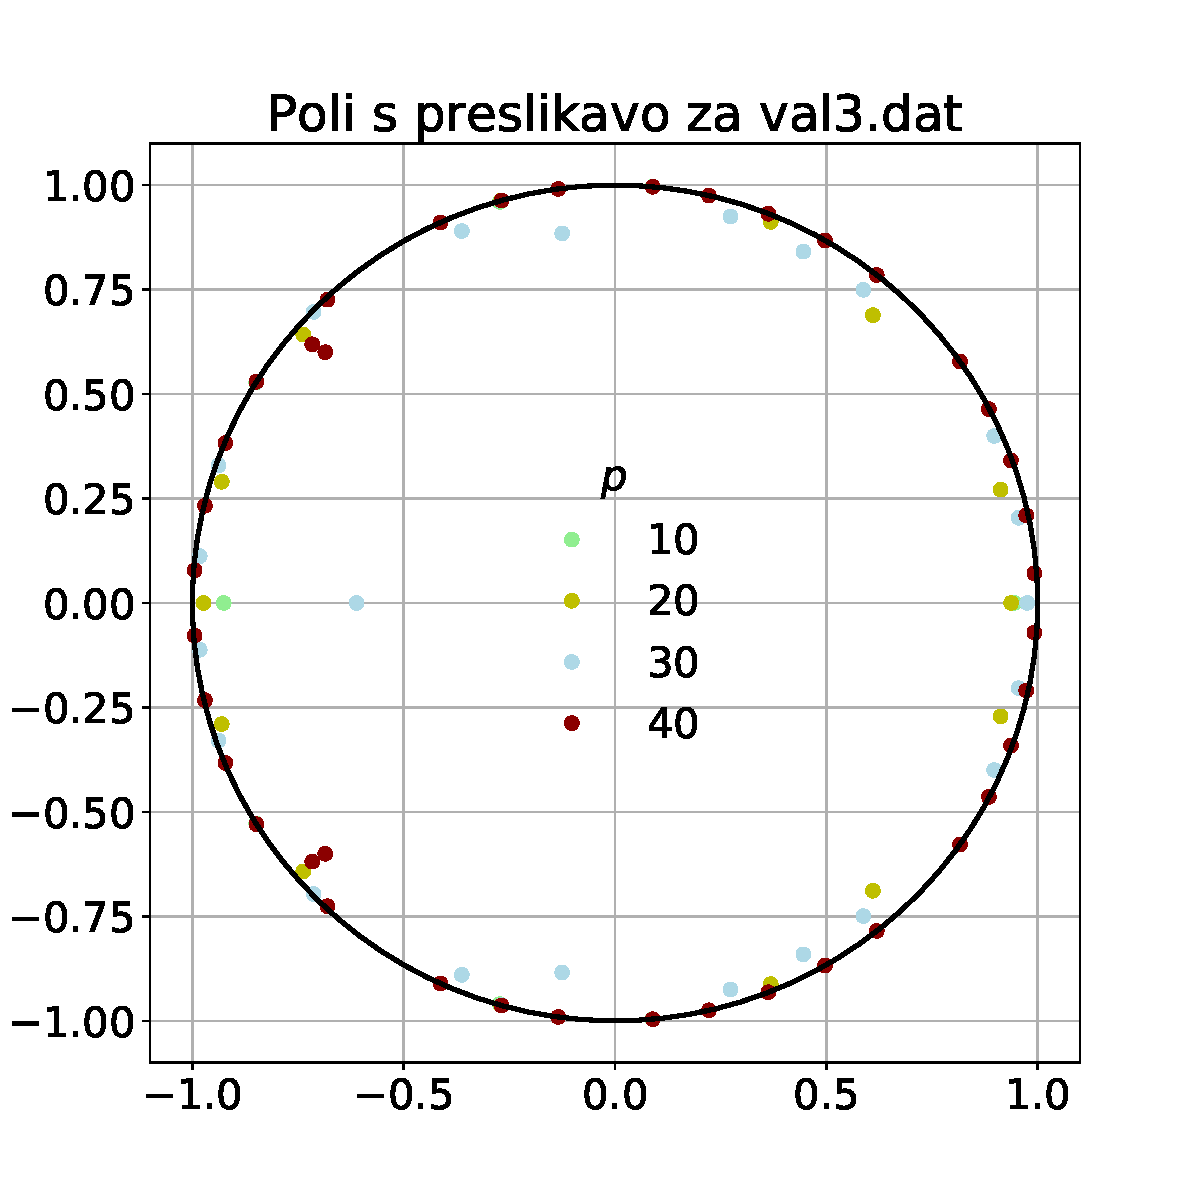
\includegraphics[width=8cm, height=5cm]{prva_primerjava2.pdf}
\caption{Vidimo, da s višanjem členov $p$ tudi več ničel pade izven enotskega kroga (levo), ki jih nato preslikamo znotraj (desno).}  
\end{figure}

\begin{figure}[H]
\centering
  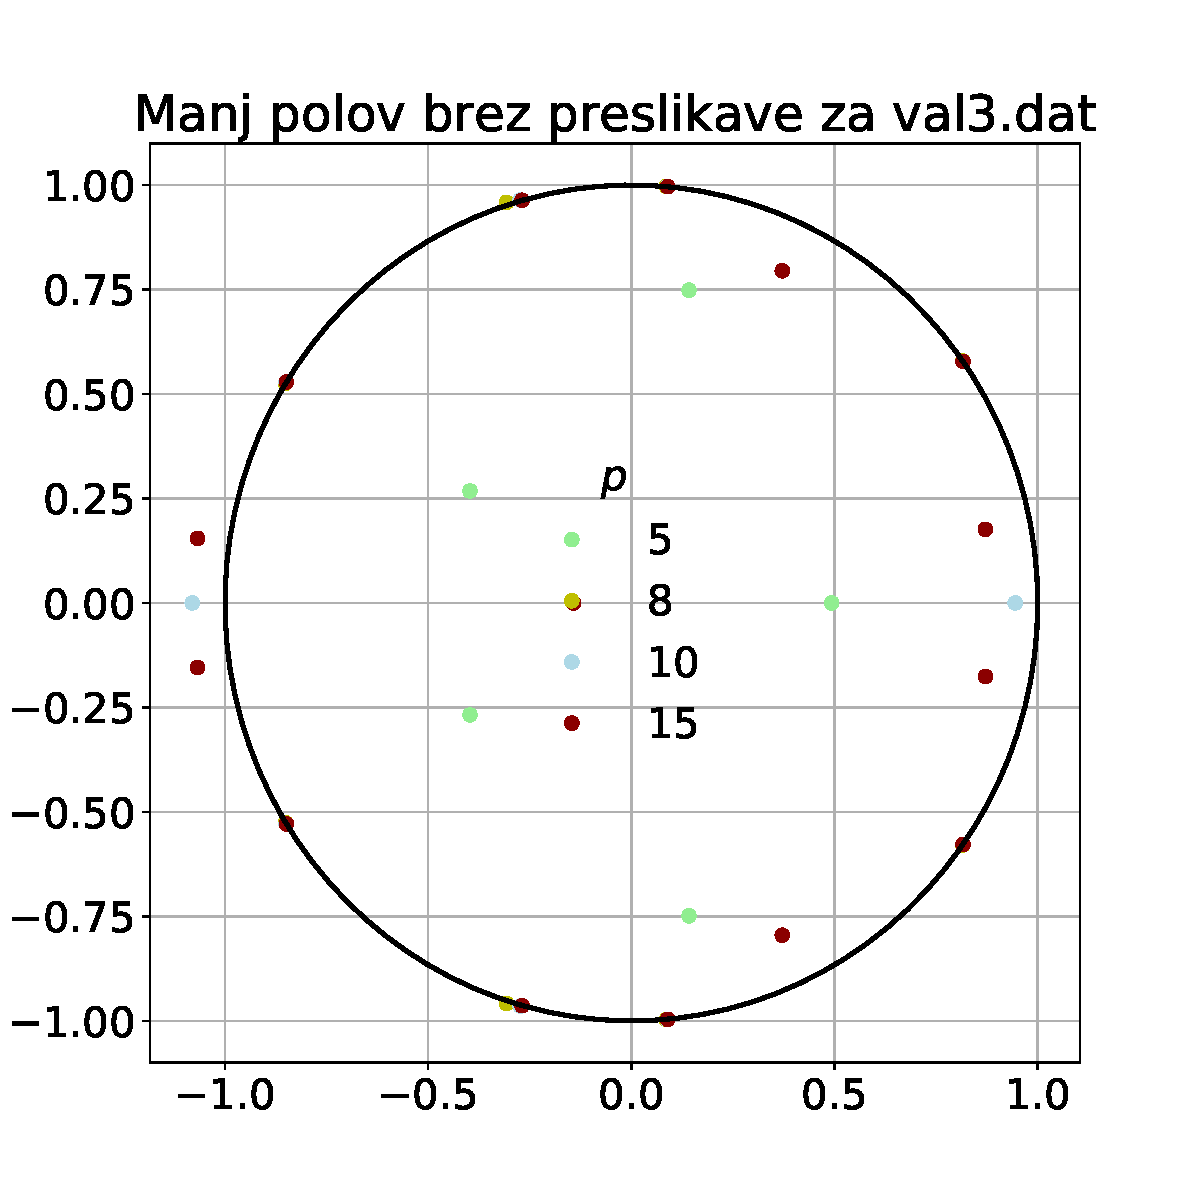
\includegraphics[width=8cm,height=5cm]{prva_primerjava3.pdf}
  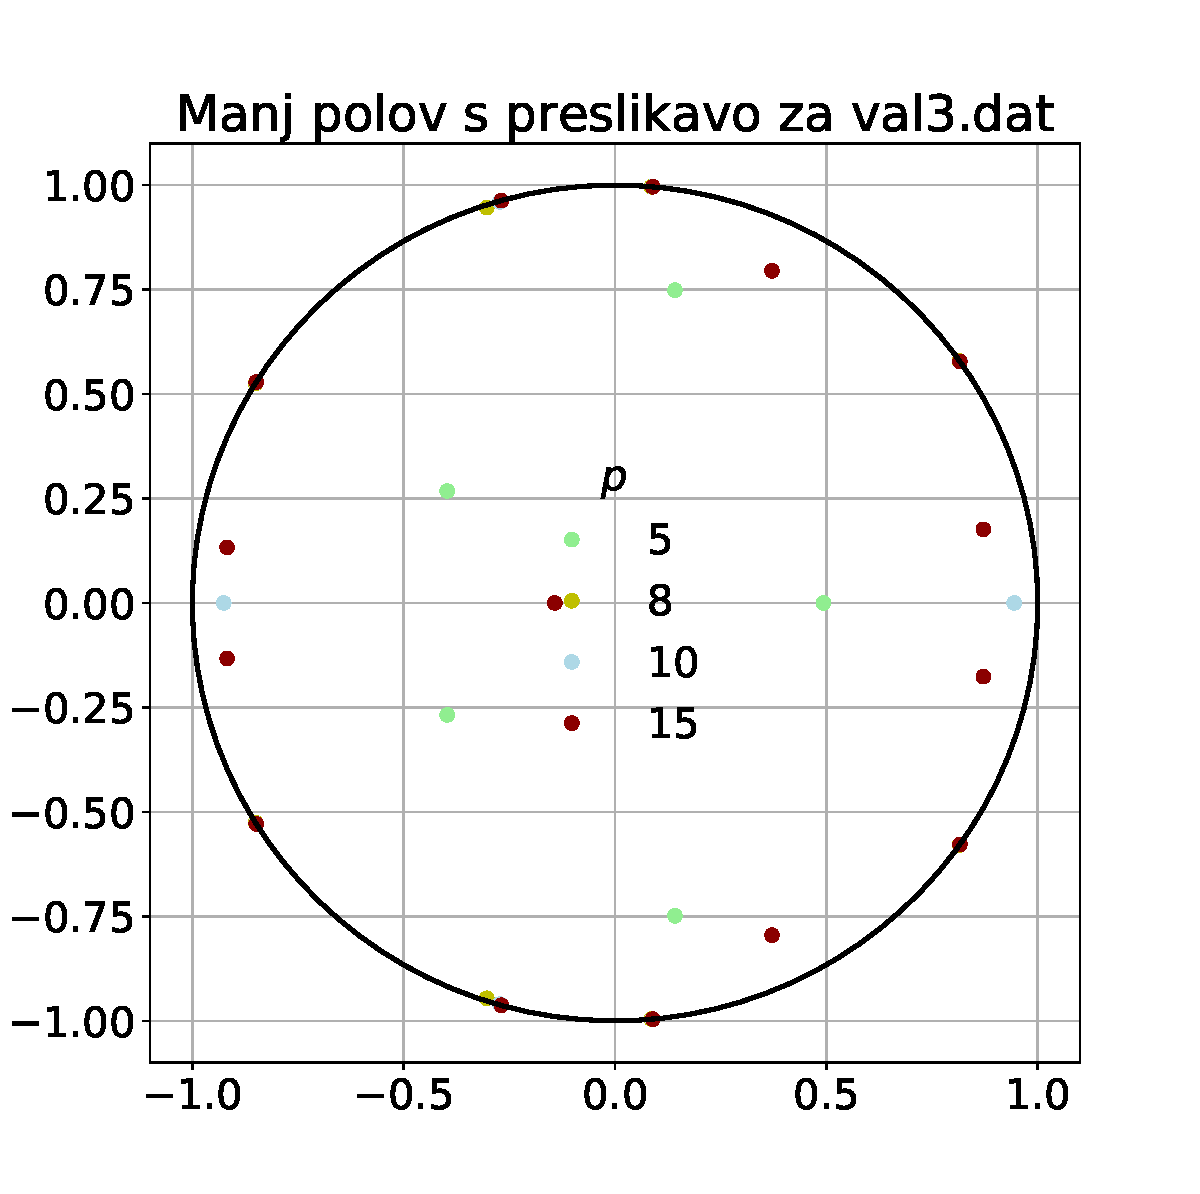
\includegraphics[width=8cm,height=5cm]{prva_primerjava4.pdf}
\caption{Pri manjših vrednostih $p$ pa izven kroga ne pade skoraj nobena ničla.}  
\end{figure}
Sedaj lahko narišemo spekter po enačbi (7)
\begin{figure}[H]
\centering
  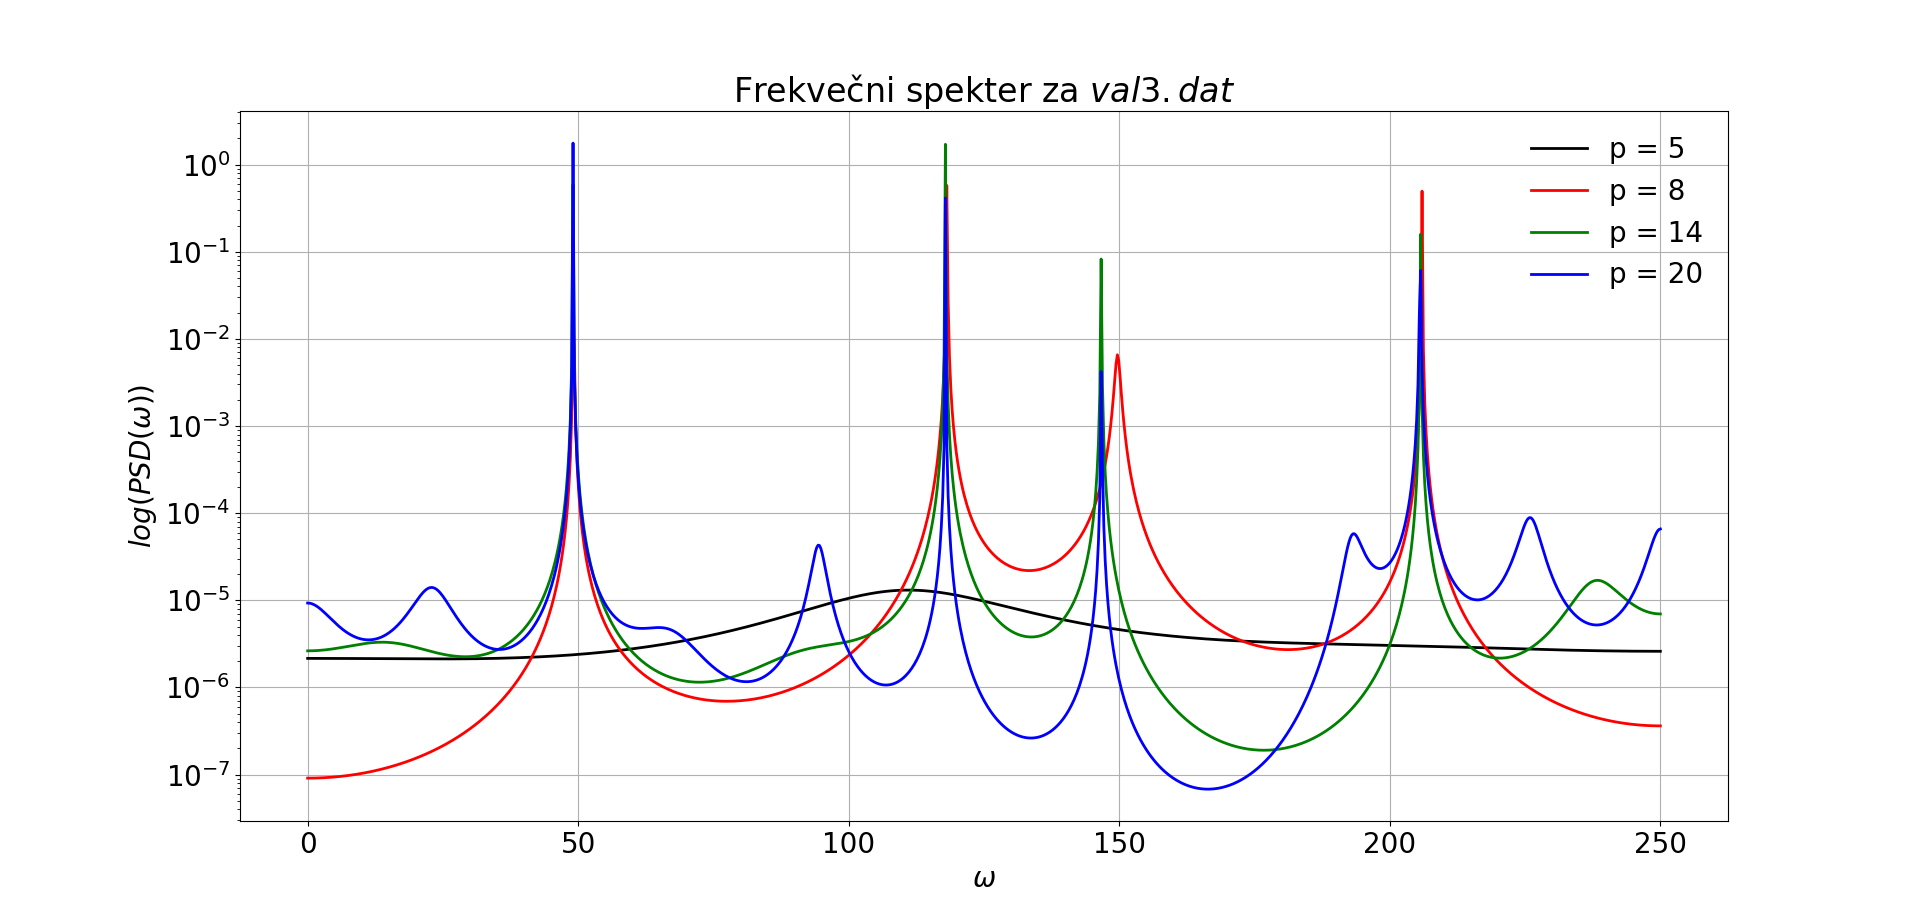
\includegraphics[width=16cm,height=5cm]{prva_frekvencni1.png}
  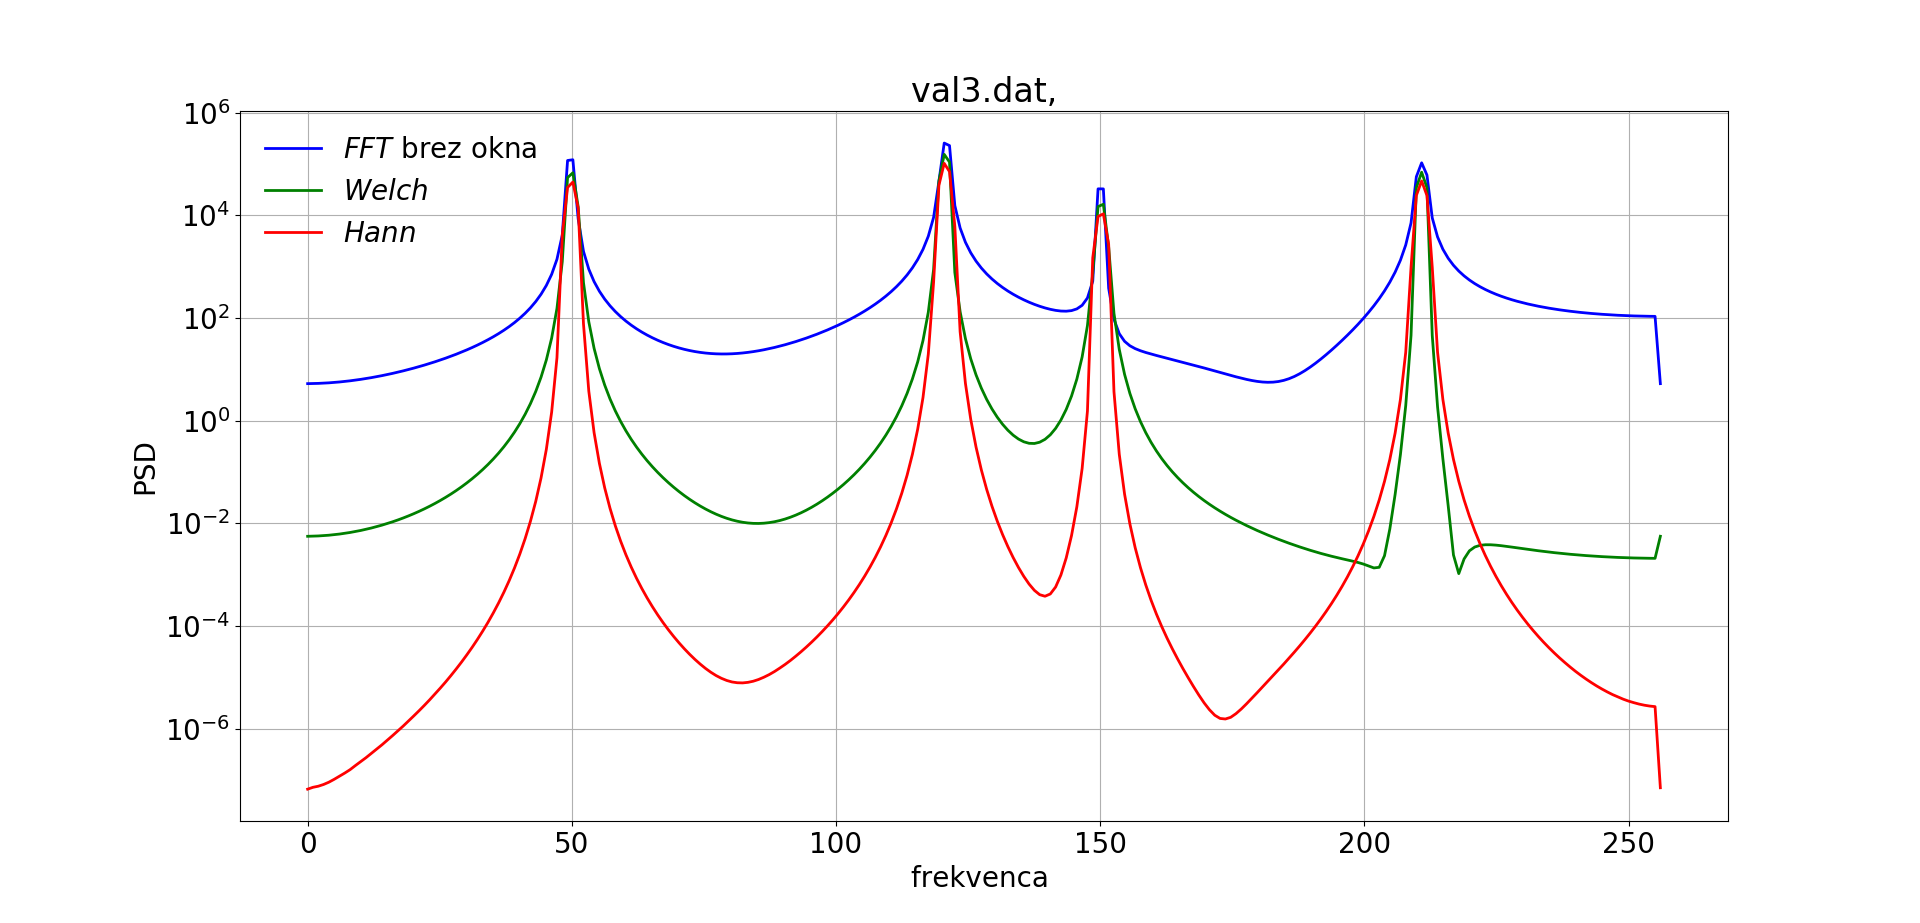
\includegraphics[width=16cm,height=5cm]{prva_tretja1b.png}
\caption{Primerjava MEM(zgoraj) in FFT (spodaj). Vidimo da se frekvenčni vrhovi ujemajo, pri čemer bi ocenili da  MEM bolj izolira vrhove in je zaradi tega ločljivost boljša. Pri višjih p dobimo več vrhov in zaradi tega zašumimo sliko. Na dani sliki je verjetno najboljši $p = 14$, čeprav se nakoncu naredi tudi vrh za šum in bi bil verjetno boljši p med 8 in 14.} 
\end{figure}
Vidimo da ima MEM metoda veliko boljšo ločljivost, vendar pa je težko uganiti koliko stopenj polinoma vzeti. Zato je verjetno najboljše narediti FFT za oceno vrhov, nato pa s MEM dobiti točno frekvenco vrha.
\begin{figure}[H]
\centering
  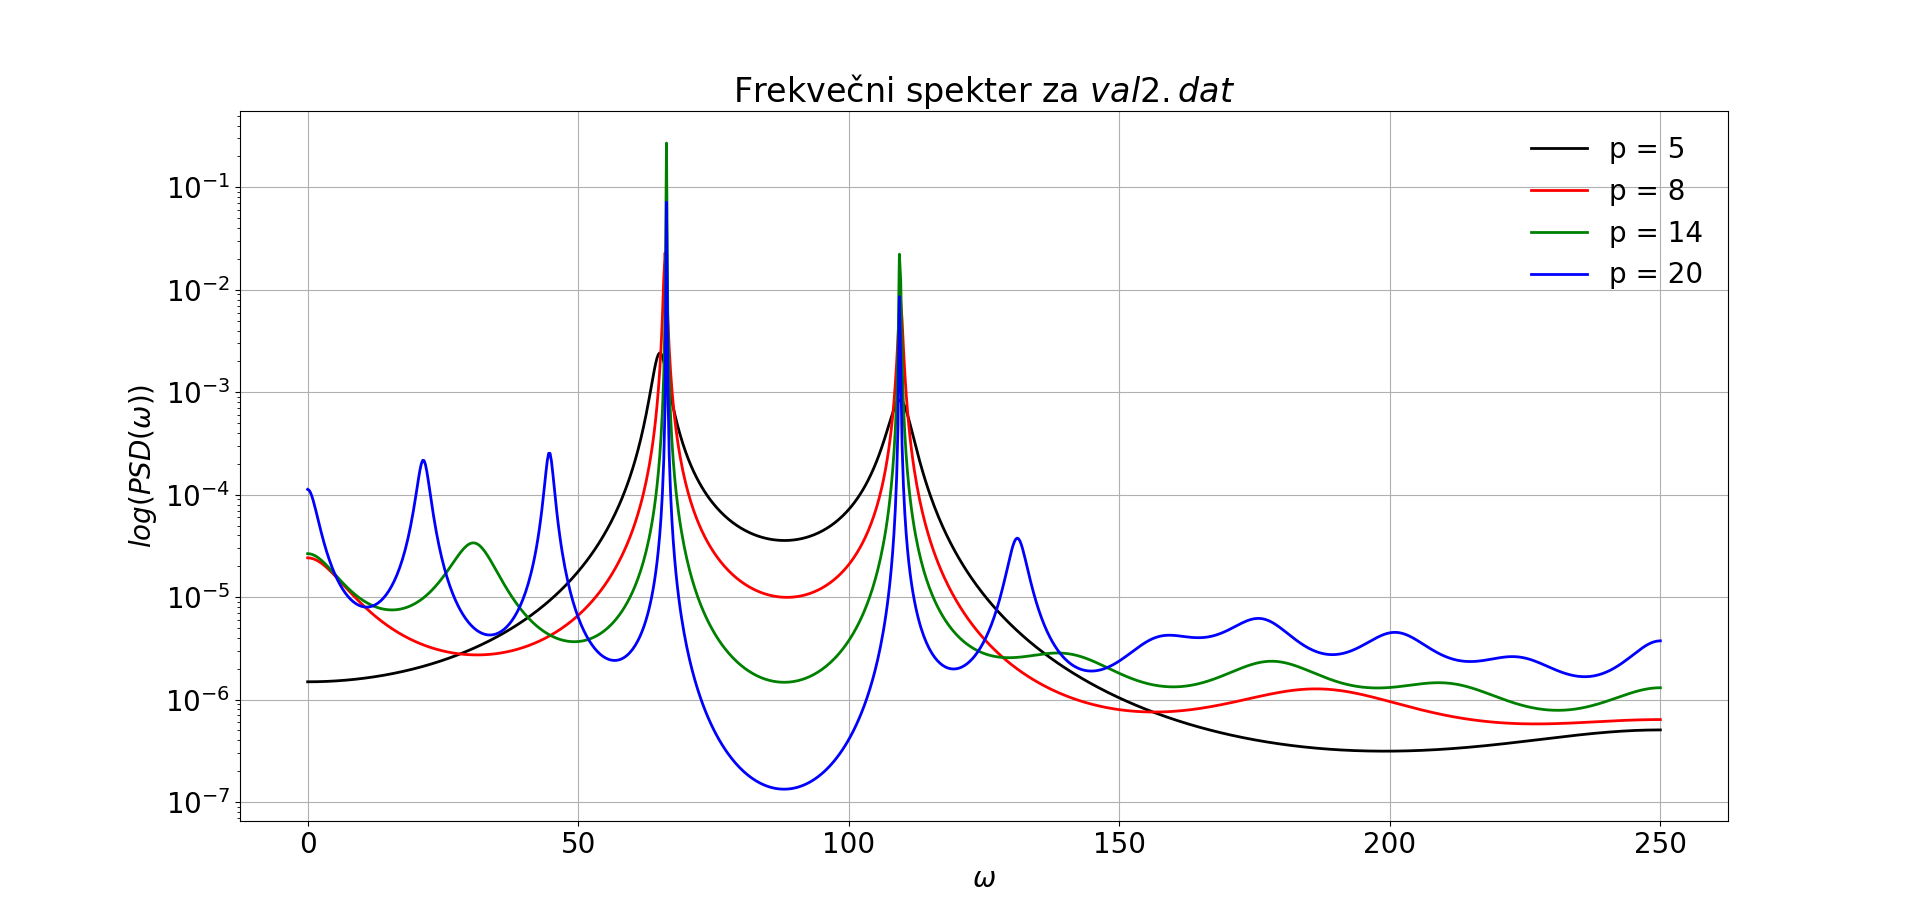
\includegraphics[width=16cm,height=5cm]{prva_frekvencni2.png}
  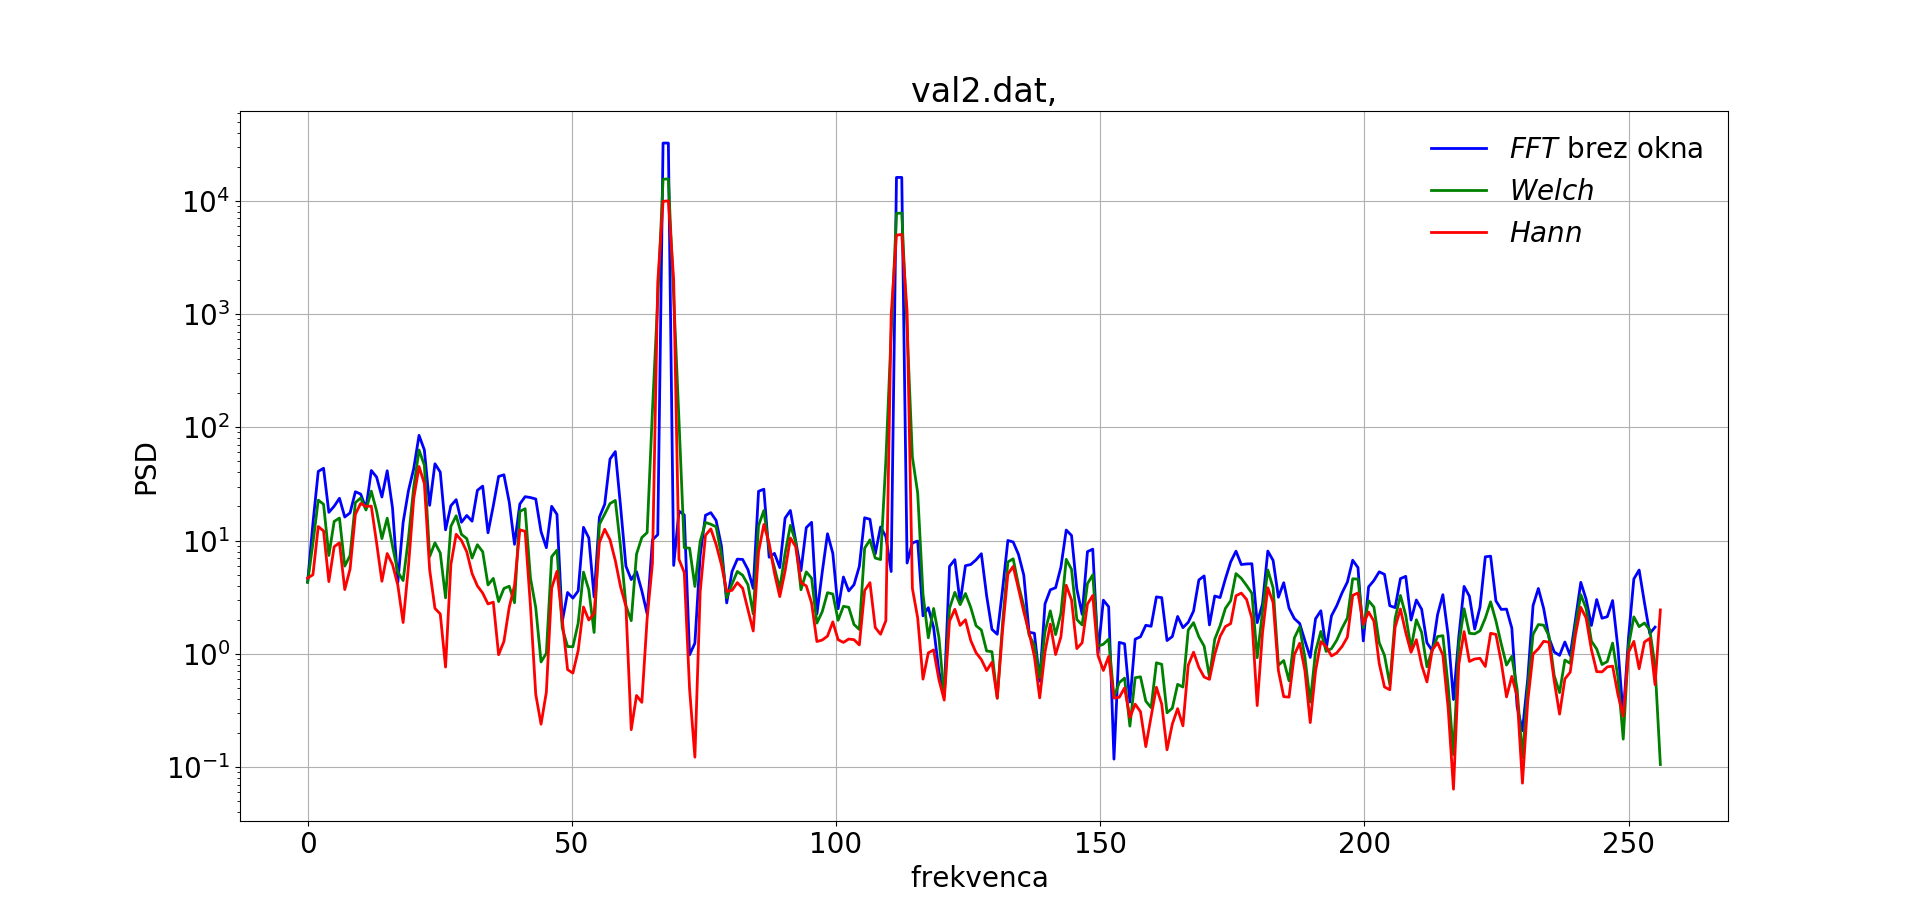
\includegraphics[width=16cm,height=5cm]{prva_tretji1.png}
\caption{Primerjava MEM (zgoraj) in FFT (spodaj). Vidimo da nam MEM pri $p=8$ da najboljši rezultat, ki ni zašumljen in zato boljši kot FFT. Ločljivost v tem primeru ni veliko boljša. Pri izboljšani ločljivosti pa dobimo že več šuma.}
\end{figure}
Verjetno je pri velikih vzorcih bolj vseeno katero metodo (MEM ali FFT) vzamemo, saj je frekvenca vzorčenja večja in zato tudi spekter bolj bogat.
\section{Značilnosti koncentracije CO2}
Poglejmo si najprej naraščanje koncentracije $CO_2$ po letih. Opazimo linearni trend naraščanja in periodičnost vmes, zato linearni trend odštejemo, saj ta ne vpliva na spektralno analizo signala.
\begin{figure}[H]
\centering
  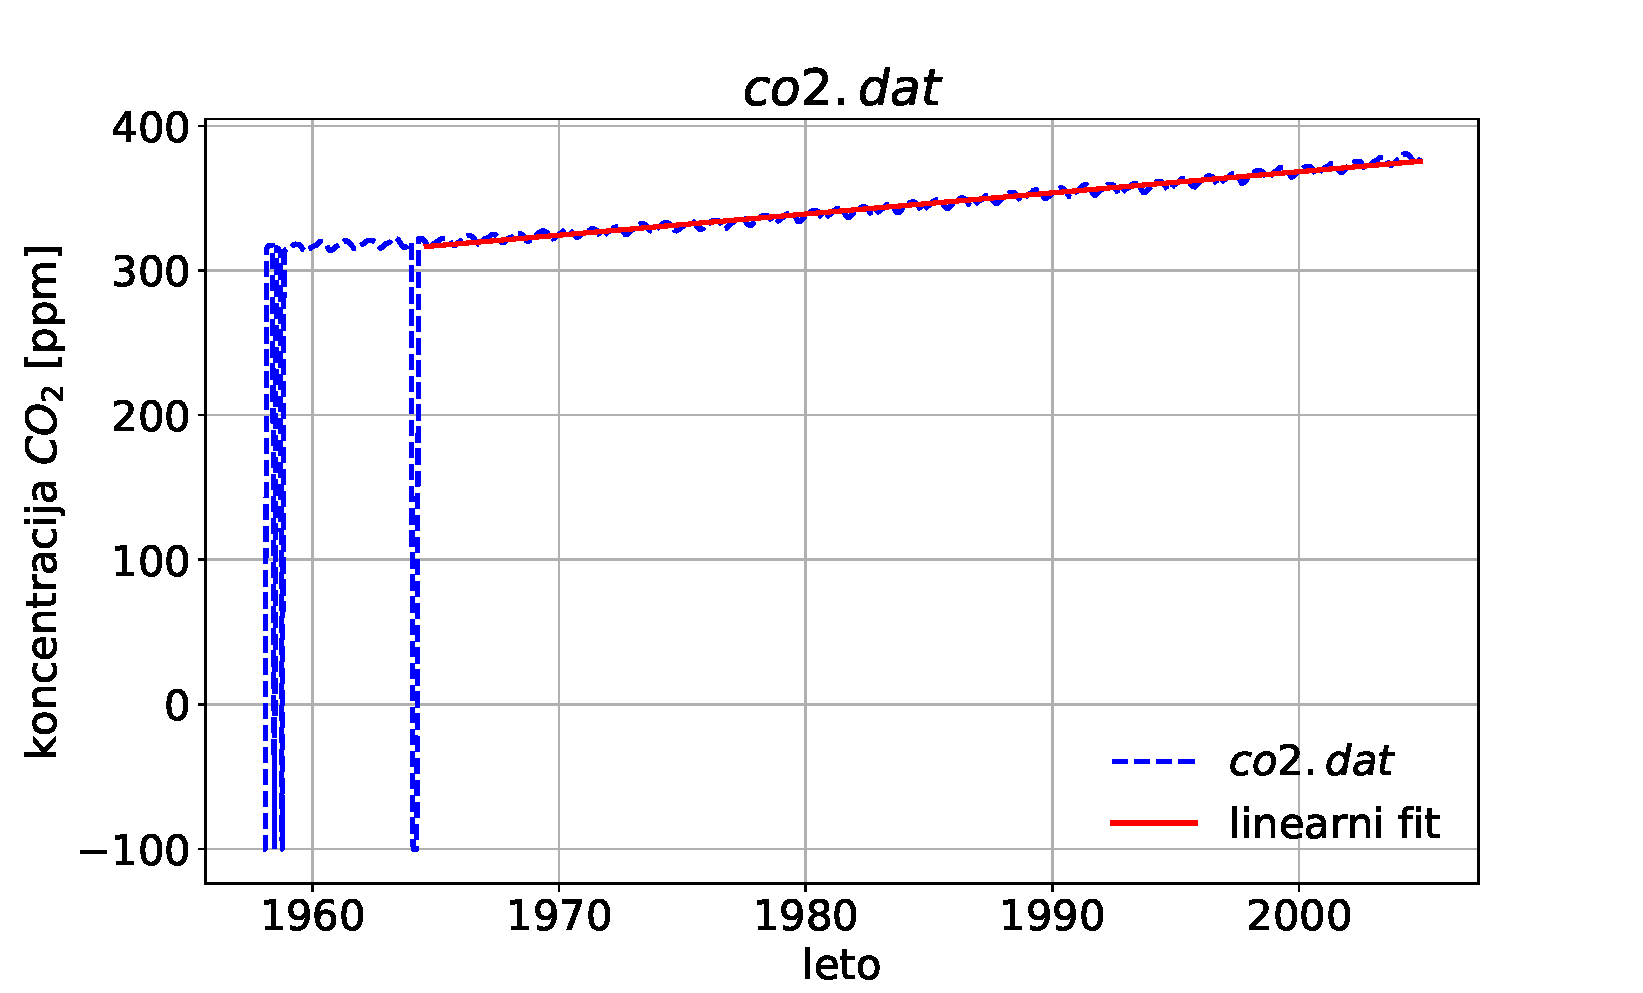
\includegraphics[width=8cm,height=6cm]{druga_prvi.pdf}
  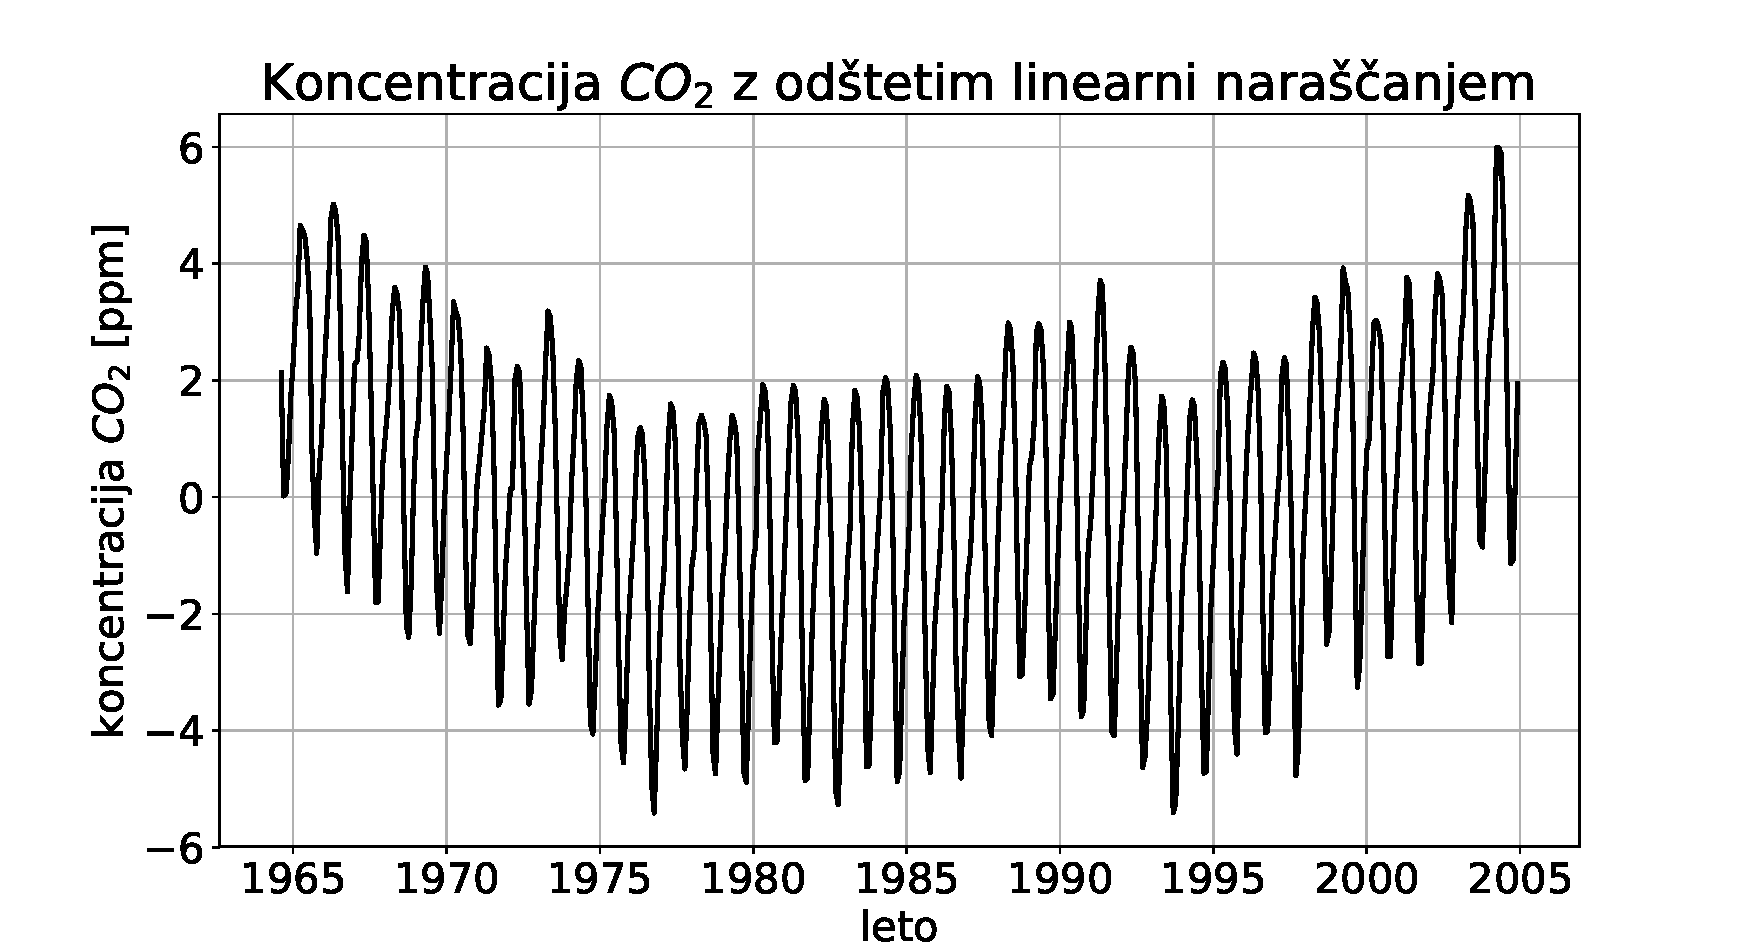
\includegraphics[width=8cm,height=6cm]{druga_prvi2.pdf}
\caption{Levo je prikaz datoteke $co2.dat$ s ustreznim fitom, in desno prikaz periodičnosti koncentracije $CO_2$.}
\end{figure}
Sedaj zopet uporabimo algoritem MEM in tako dobimo frekvenčni spekter.
\begin{figure}[H]
\centering
  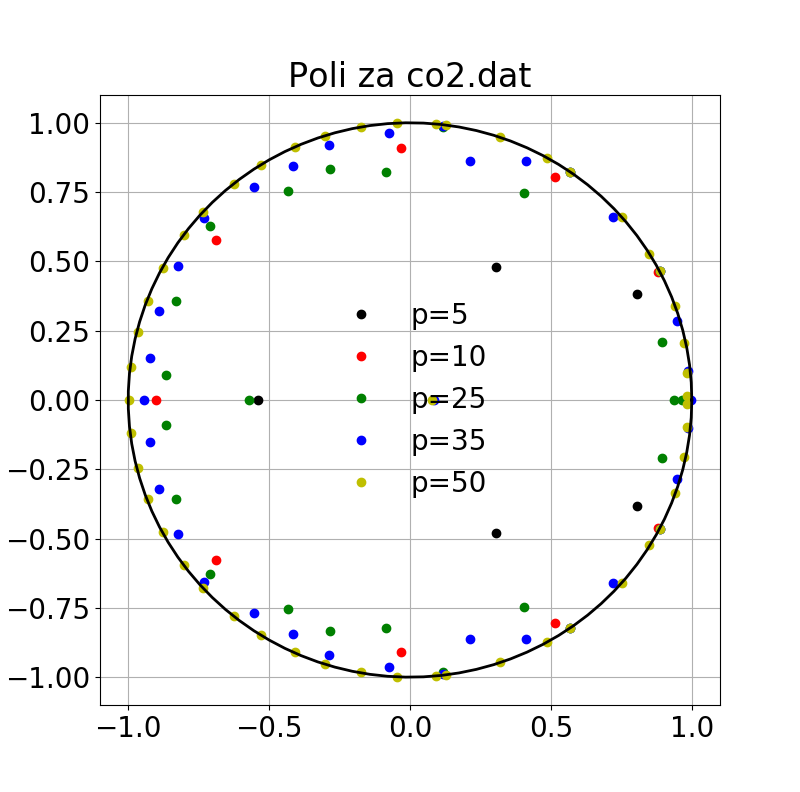
\includegraphics[width=8cm,height=6cm]{prva_drugi3.png}
  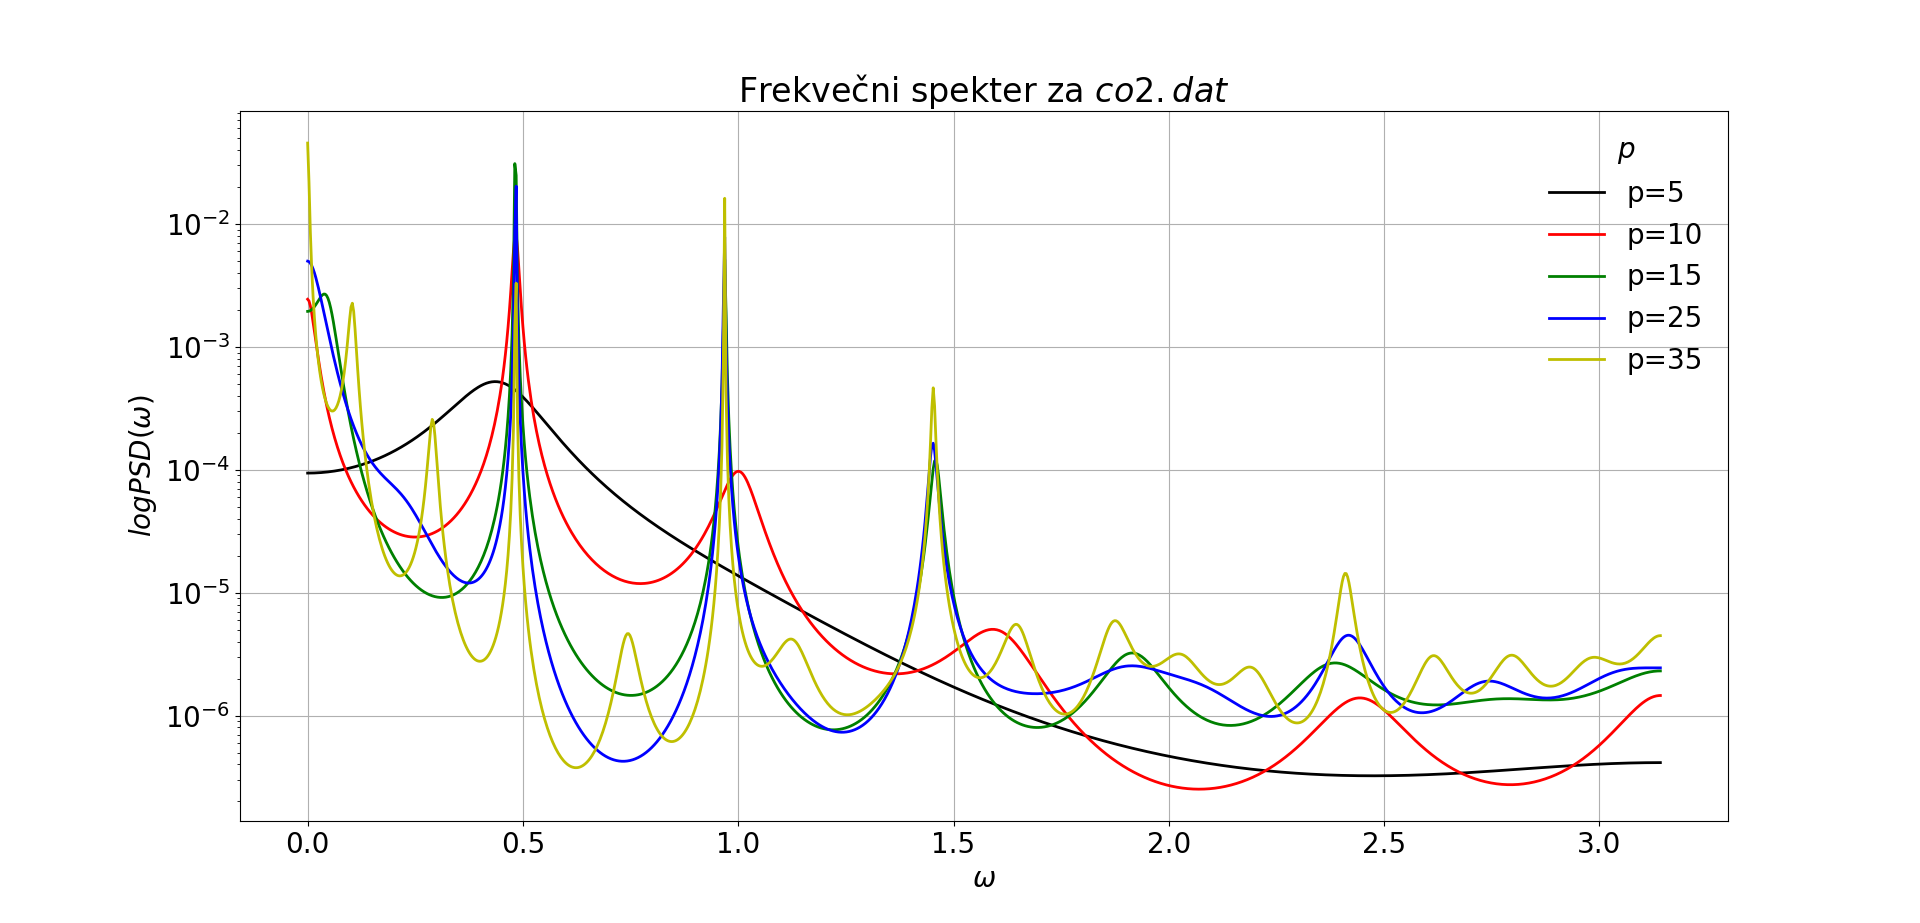
\includegraphics[width=18cm,height=6cm]{druga_frekvencni.png}
  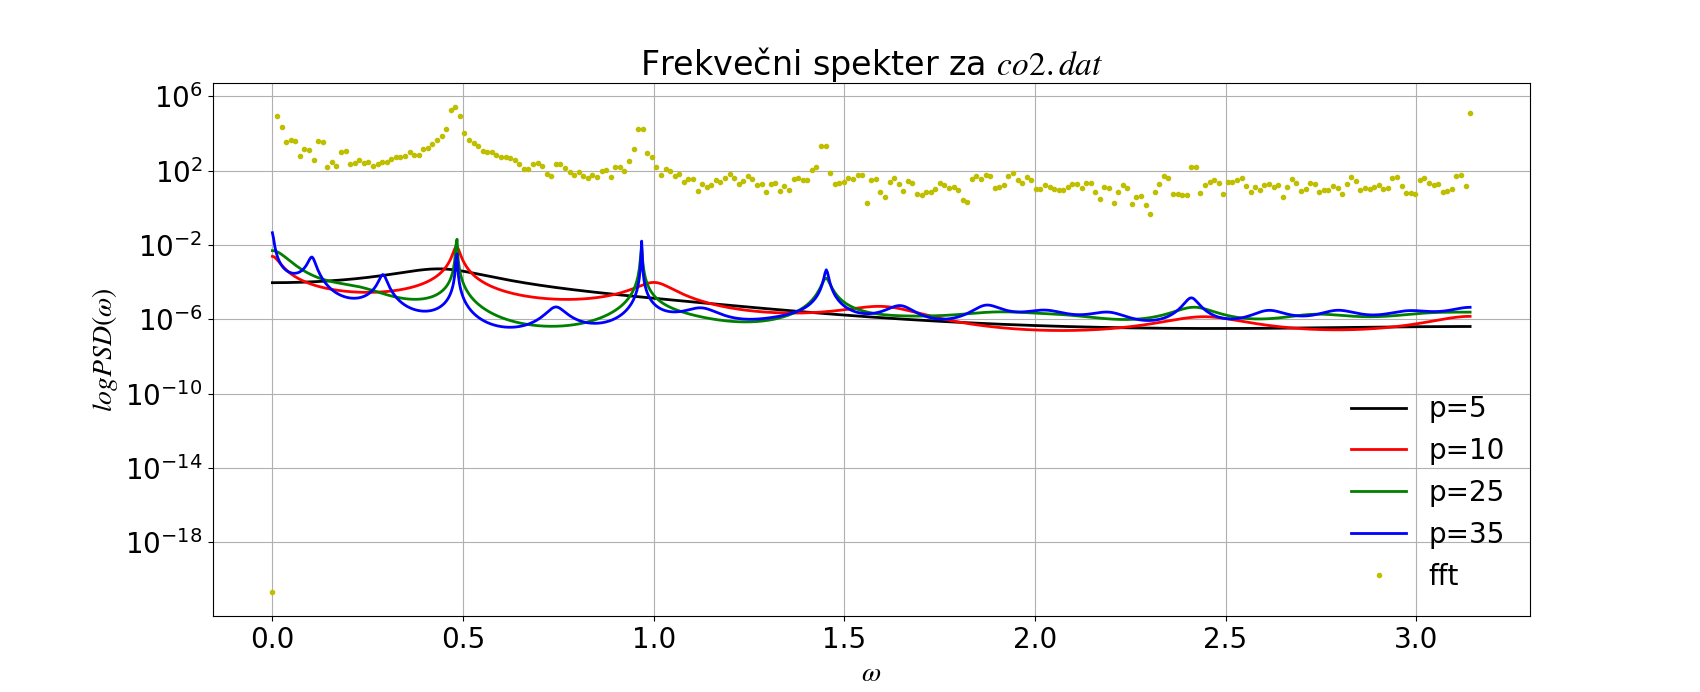
\includegraphics[width=18cm,height=6cm]{prva_drugi4b.png}
  
\end{figure} 
Poli in spekter za signal $co2.dat$. Vidimo da s naraščanjem polov, ti vse bolj sovpadajo na enotsko krožnico. (zgoraj). \newline
Spodaj je prikazan frekvenčni spekter za $p = 5,10,15,25,35$. Pri višanju $p$ zopet dobimo več šuma, zanimivo pa nam p=10 ne zadane frekvence $\sim 1.4 $. Tako bi za najboljšo rešitev vzeli $p=25$. Za vrh pri frekvenci 2.5 nisem siguren ali je le šum saj bi pri višjih p=35 (rumena) vrh moral biti bolj izrazit. FFT ustreza frekvencni sliki (spodaj) le da so frekvence manj ostre. Tako so glavne frekvence :
\begin{table}[H]
\centering
\caption{Frekvece vrhov}
\label{my-label}
\begin{tabular}{llll}
$\omega$ & 0.5 & 0.8 & 1.4
\end{tabular}
\end{table}
\section{Občutljivost MEMS na  razločevanje bližnjih vrhov. }
Vzemimo signal
\begin{equation}
s(t) = sin(2\pi t) + sin(2\pi t + \Delta \omega)
\end{equation}
Sedaj spremnijamo fazni zamik $\Delta \omega$ in opazujemo ločljivost MEM.

\begin{figure}[H]
\centering
  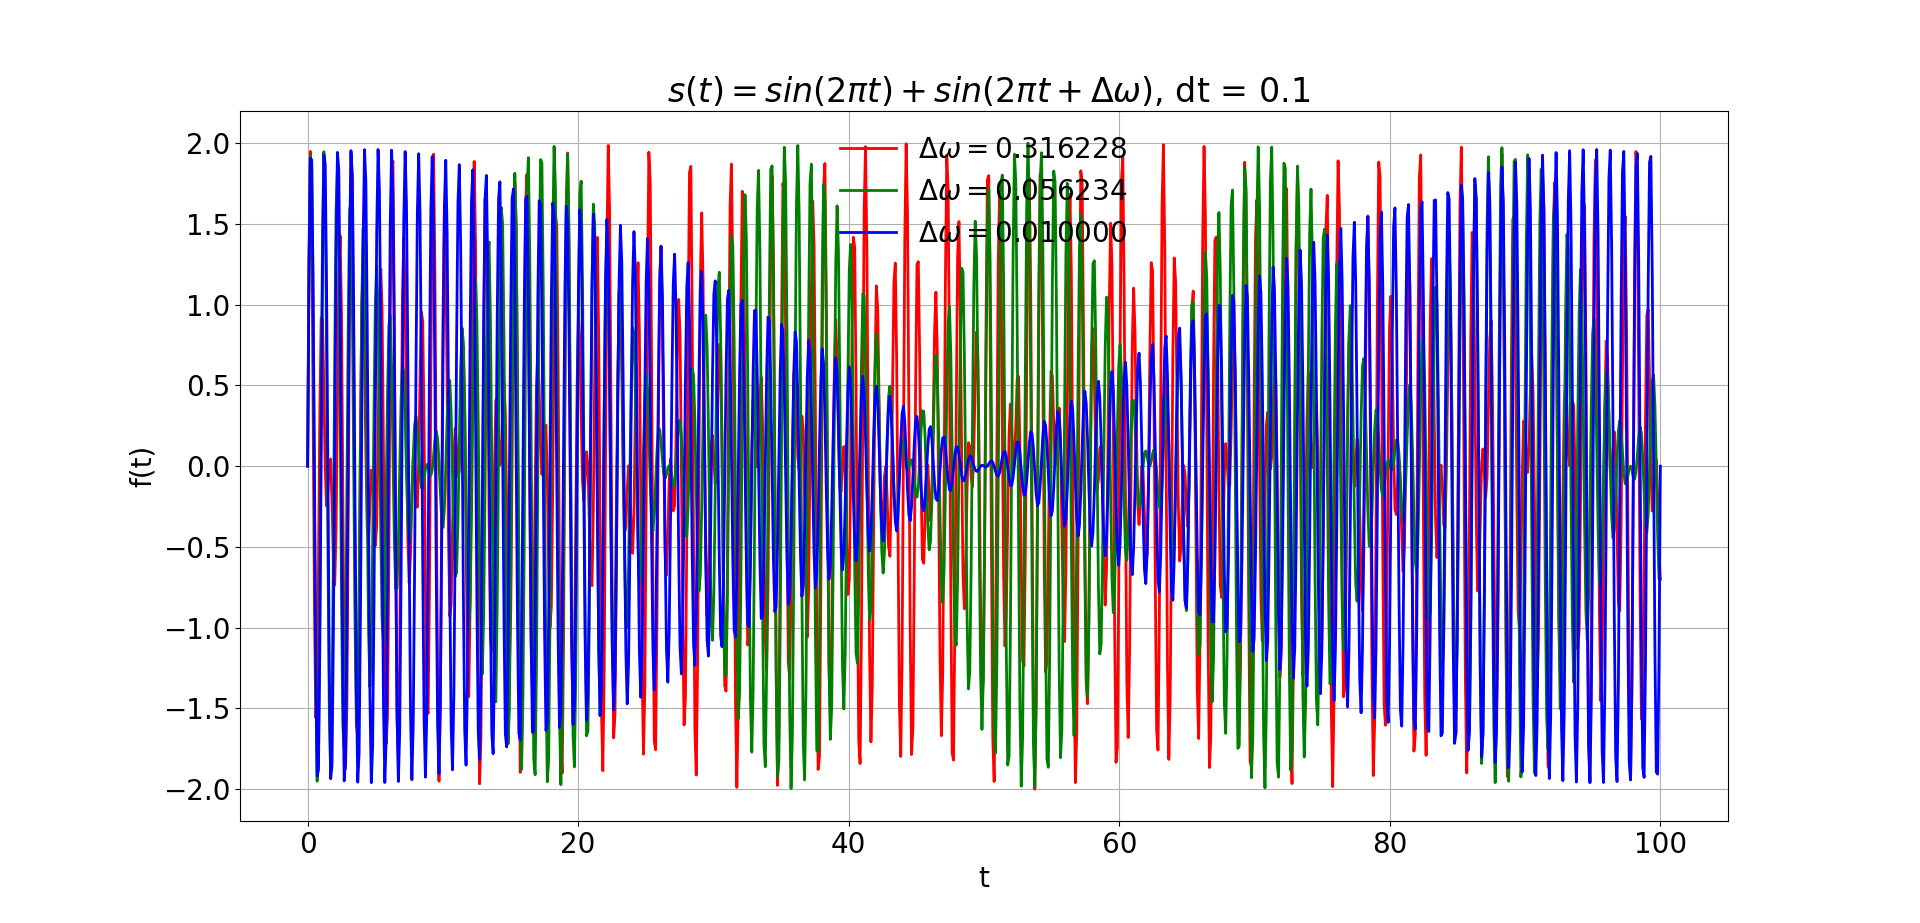
\includegraphics[width=16cm,height=5cm]{prva_cetrti.png}
  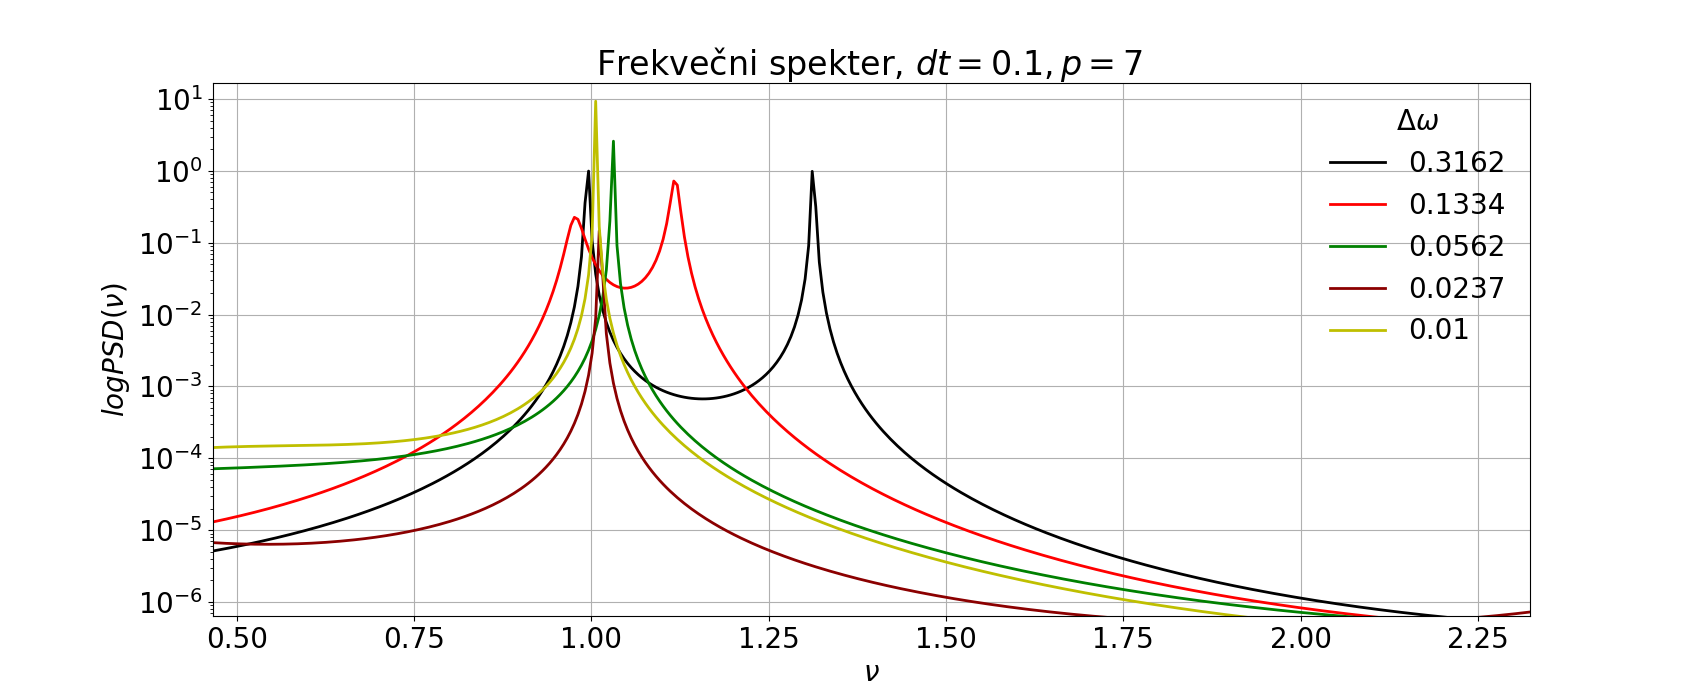
\includegraphics[width=16cm,height=5cm]{prva_cetrti2.png}
\caption{Vidimo, da na ustezni frekvenčni skali vzamemo frekvenco $\nu = 1 Hz$ in $\nu = 1 Hz + \Delta \omega$. Ustezen vrh dobimo tako pri $1 Hz$. Vidimo da pri zamiku 0.3 Hz še opazimo dva vrhova, pri zamiku 0.13 tudi, pri zamiku $\Delta \omega \sim 0.05$ pa ne več, tako da ocenimo da je resolucija $\frac{\Delta \omega }{\omega  } = 0.05 = 5 \% $.}
\end{figure}
\section{Napovedovanje s metodo MEM}
Ko enkrat poznamo koeficiente, lahko napovedujemo signale v prihodnosti. Poglejmo si kako zares deluje na podlagi nekaj testnih primerov
\subsection{Napovedovanje CO2}
\begin{figure}[H]
\centering
  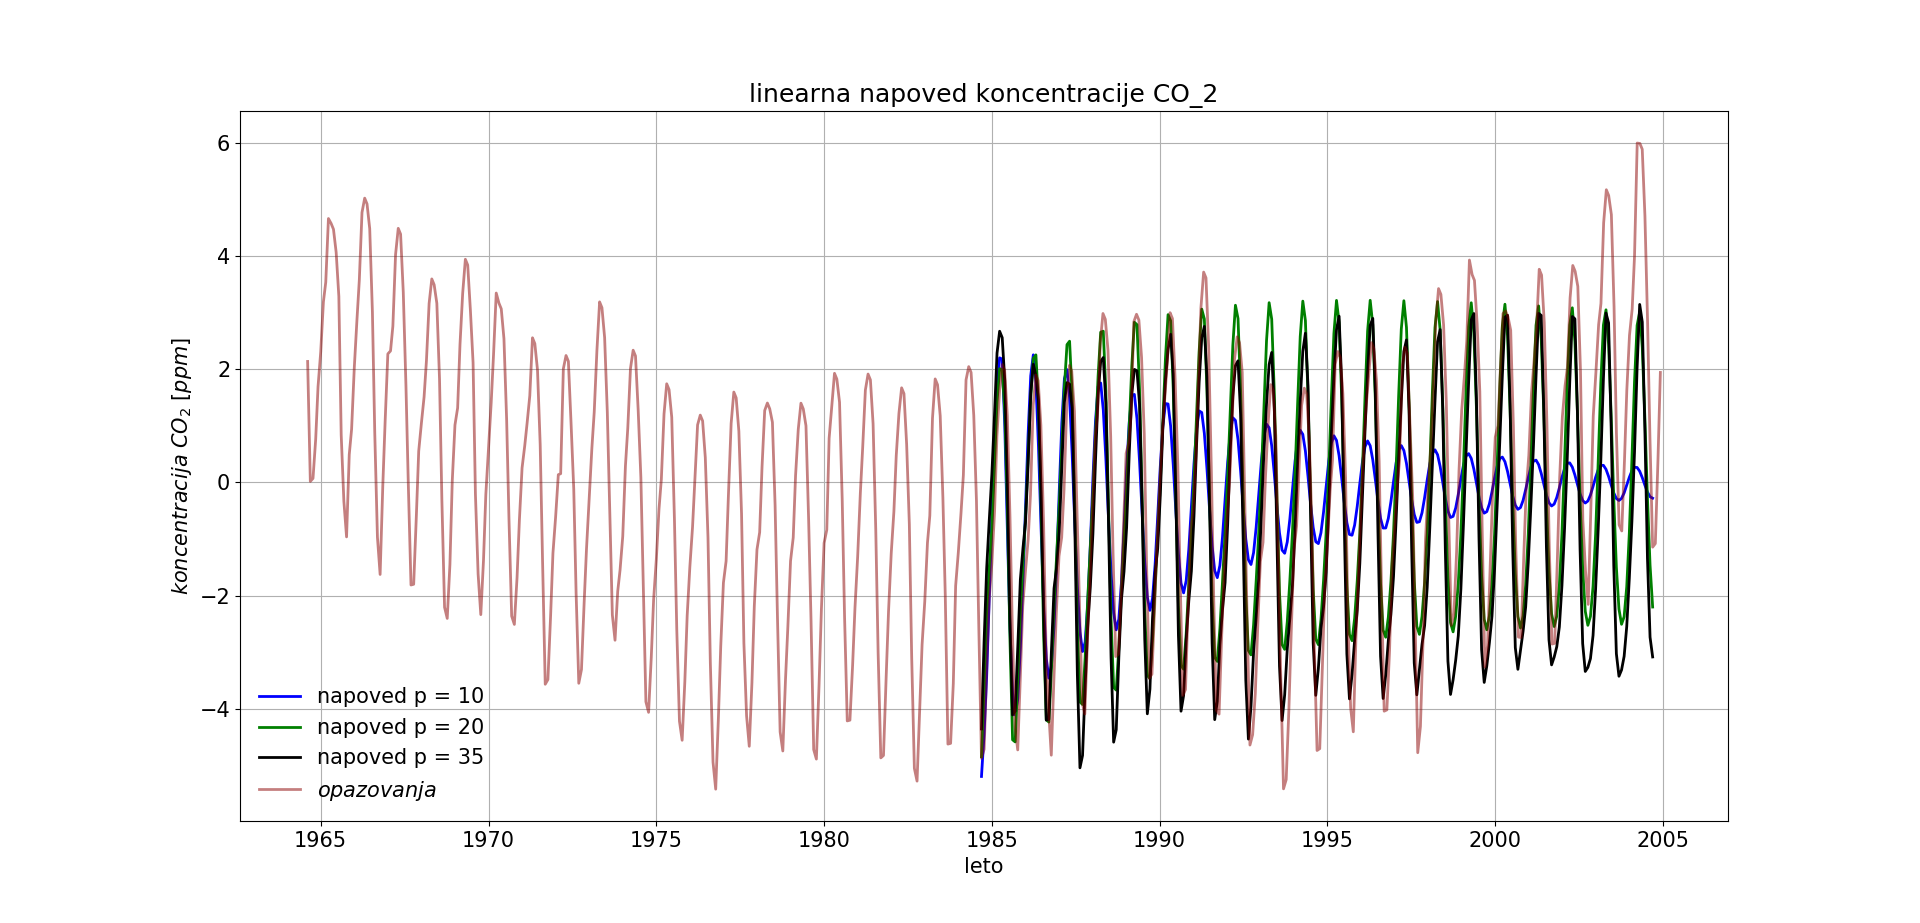
\includegraphics[width=16cm,height=6.5cm]{linearna_napoved1.png}

\caption{Linearno napovedovanje koncentracije CO2 je odvisno od števila polov ki jih vzamemo. Na grafu vidimo da je verjetno najboljša rešitev s $p=20$. Torej ne smemo vzeti ne preveč ne premanj polov. Če jih vzamemo močno preveč pa nam napoved zdivergira.}
\end{figure}

\subsection{Napovedovanje borze}
Zanima nas ali je mogoče napovedovati borzo, poglejmo si najprej pole in frekvenčni spekter datoteke $borza.dat$. Vidimo da ne opzaimo zares kakšnih vrhov , zato sklepamo da napovedovanje ne bo mogoče.
\begin{figure}[H]
\centering
  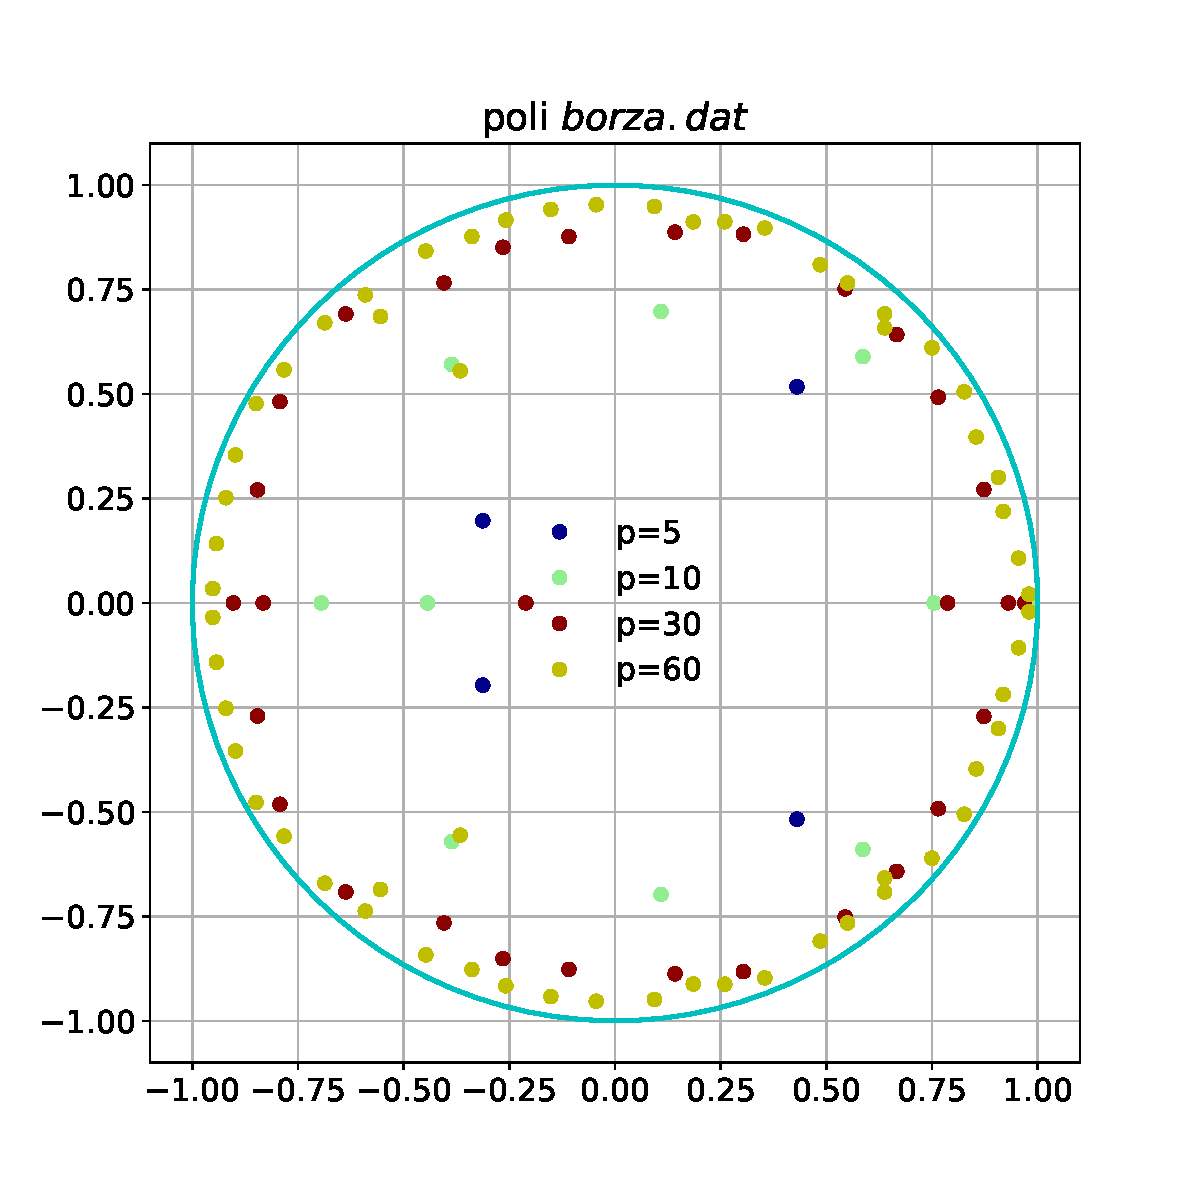
\includegraphics[width=8cm,height=5cm]{linearna_napoved3.pdf}
  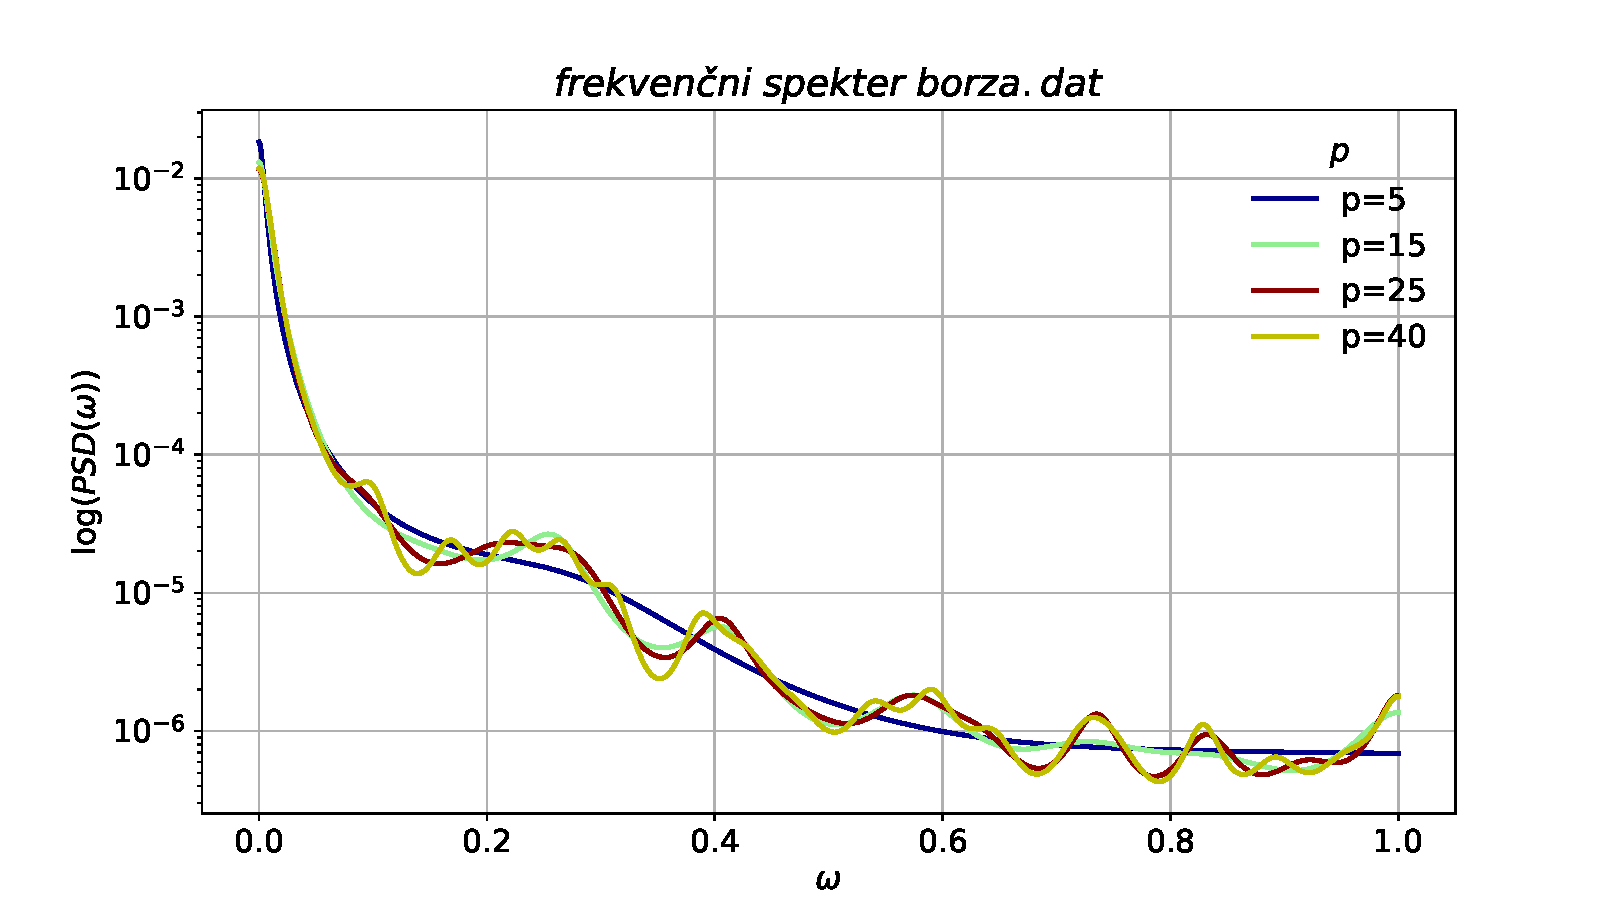
\includegraphics[width=8cm,height=5cm]{linearna_napoved4.pdf}

\end{figure}
\begin{figure}[H]
\centering
  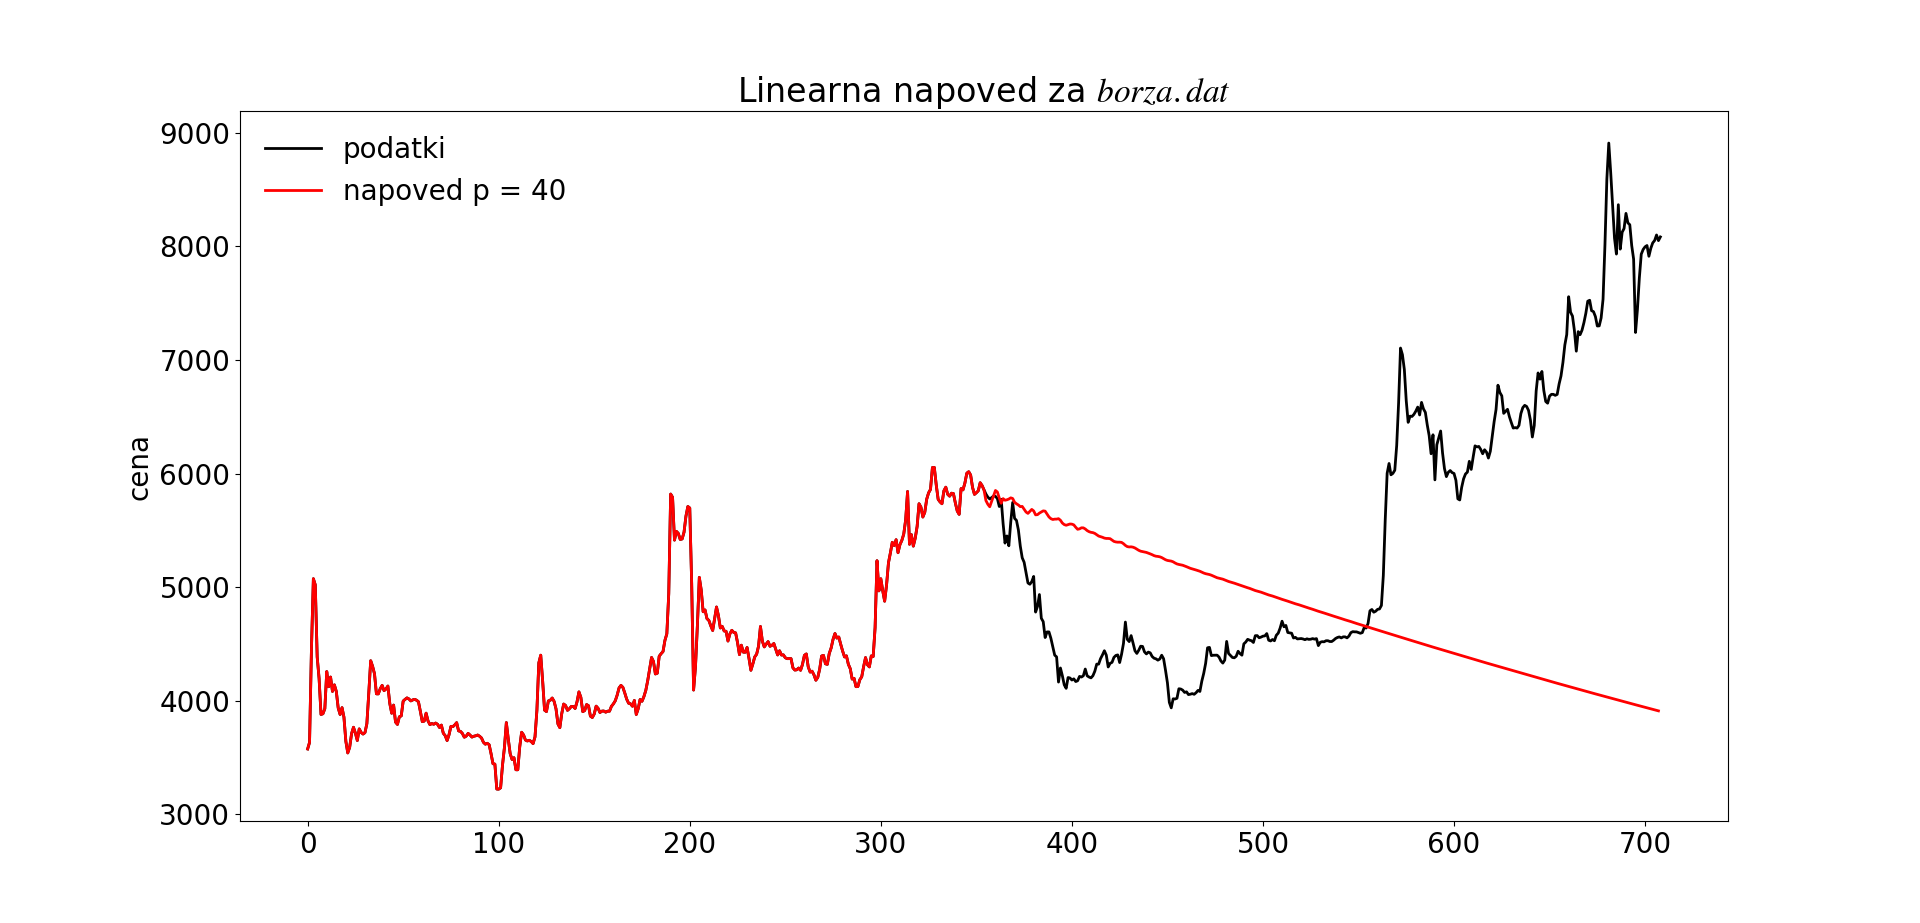
\includegraphics[width=16cm,height=6.5cm]{linearna_napoved5.png}
 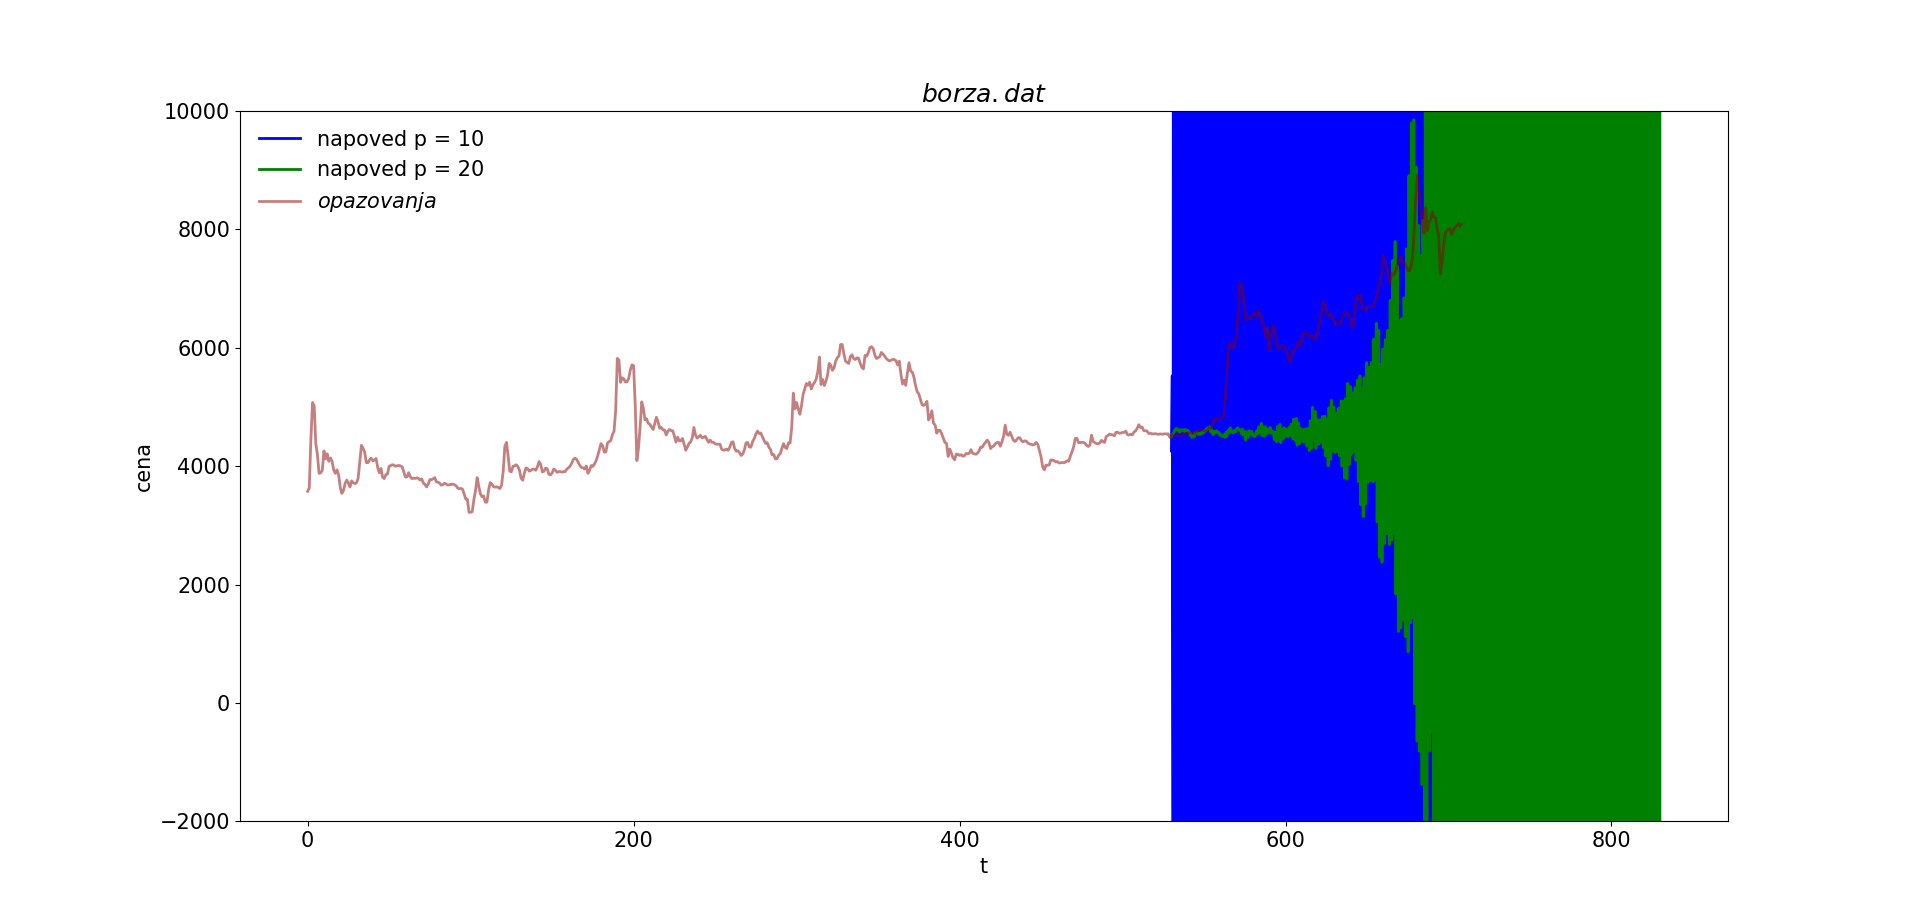
\includegraphics[width=16cm,height=6.5cm]{divergira.png}
\caption{Poskus linearne napovedi za p = 40 nam ne da zadovoljivih rezultatov. Za višje $p$ nam napoved zdivergira}
\end{figure}

\subsection{Lunine efemeride}
Ogledali smo si lunine efemeride, oziroma položaj lune v odvisnosti od časa. Podatki so bili dani v obliki rektascenzije in deklinacije. Rektascenzija se meri v urah in ima periodo 24 h, tako da sem tem podatkom prištel 24h pri vsakem obratu. Oglejmo
si linearno napoved.
\begin{figure}[H]
\centering
  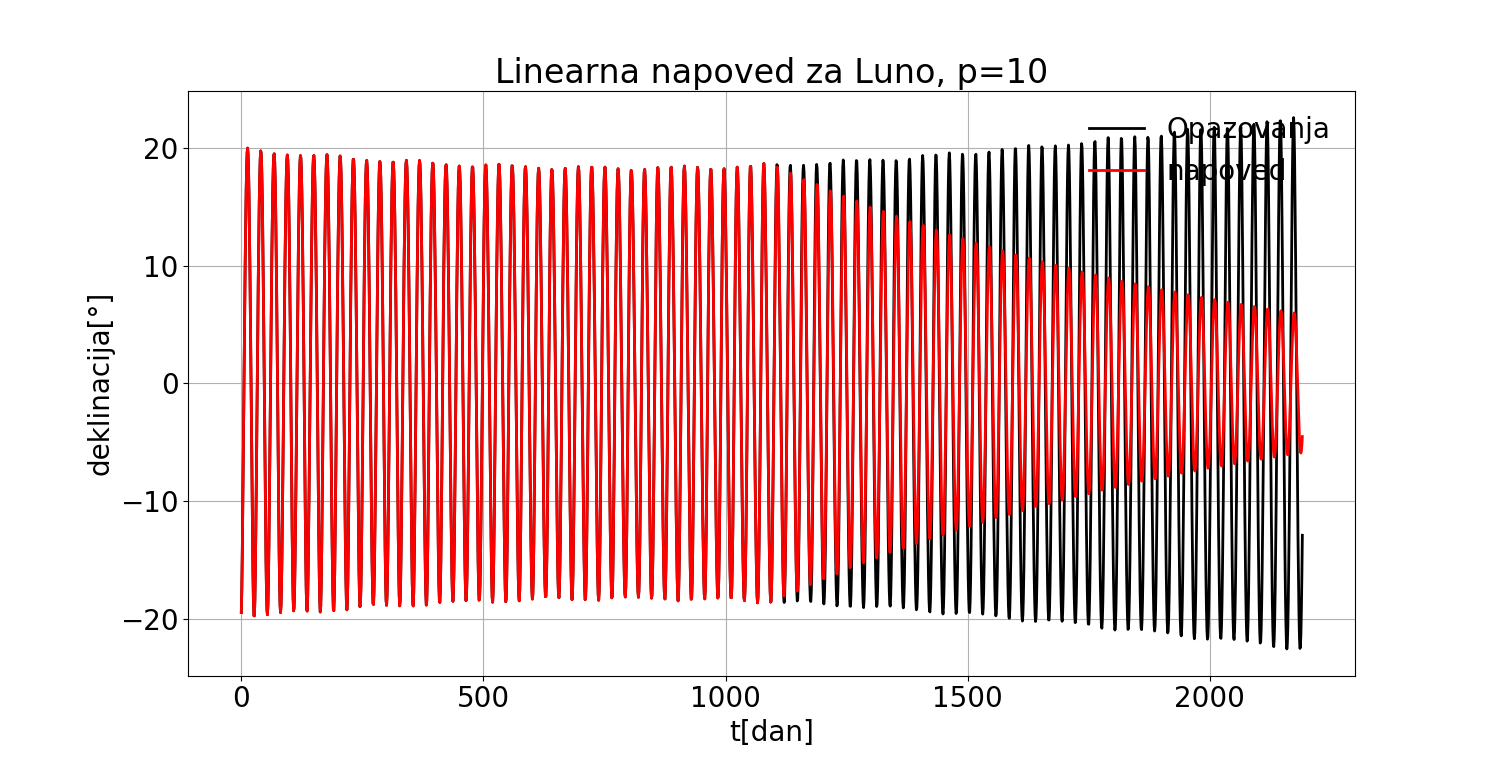
\includegraphics[width=8cm,height=5cm]{1.png}
  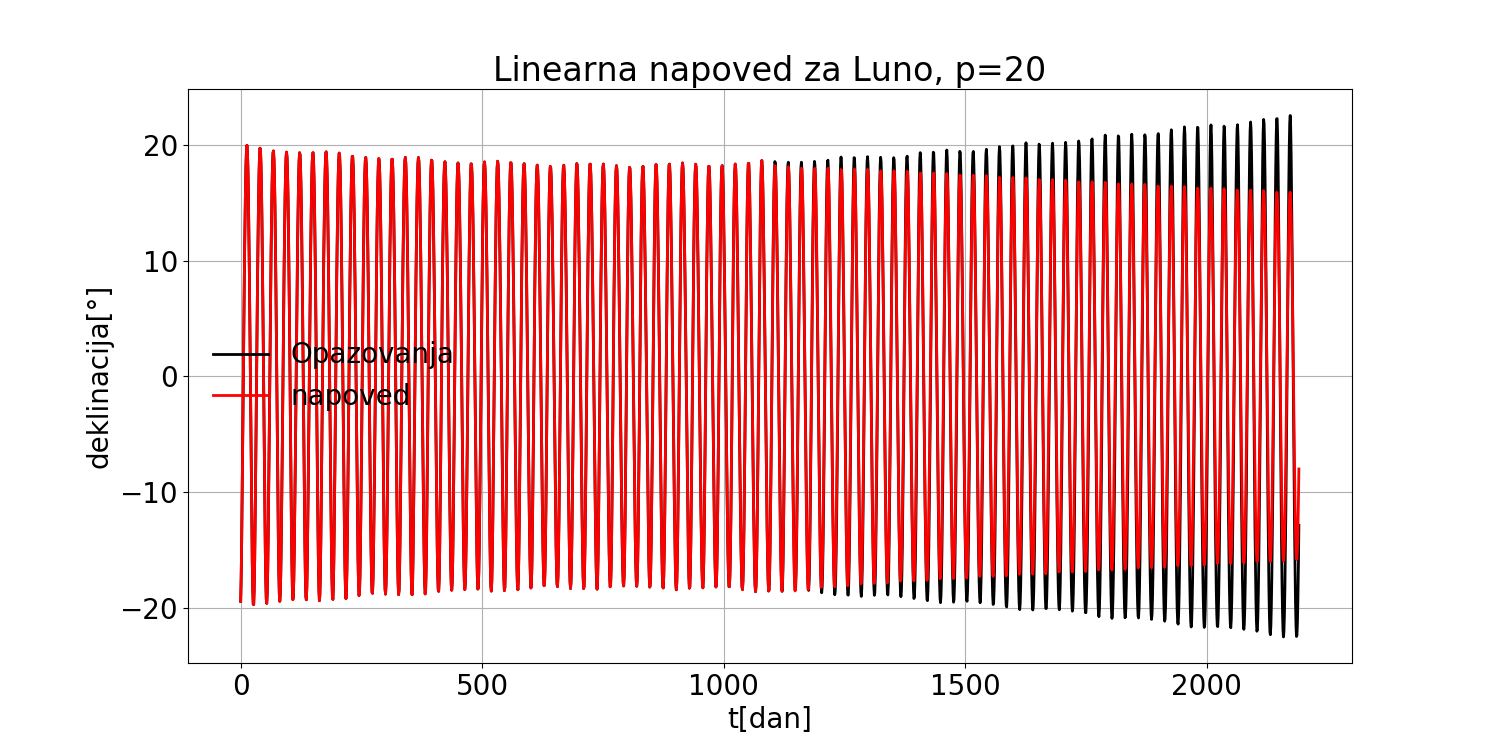
\includegraphics[width=8cm,height=5cm]{3.png}
  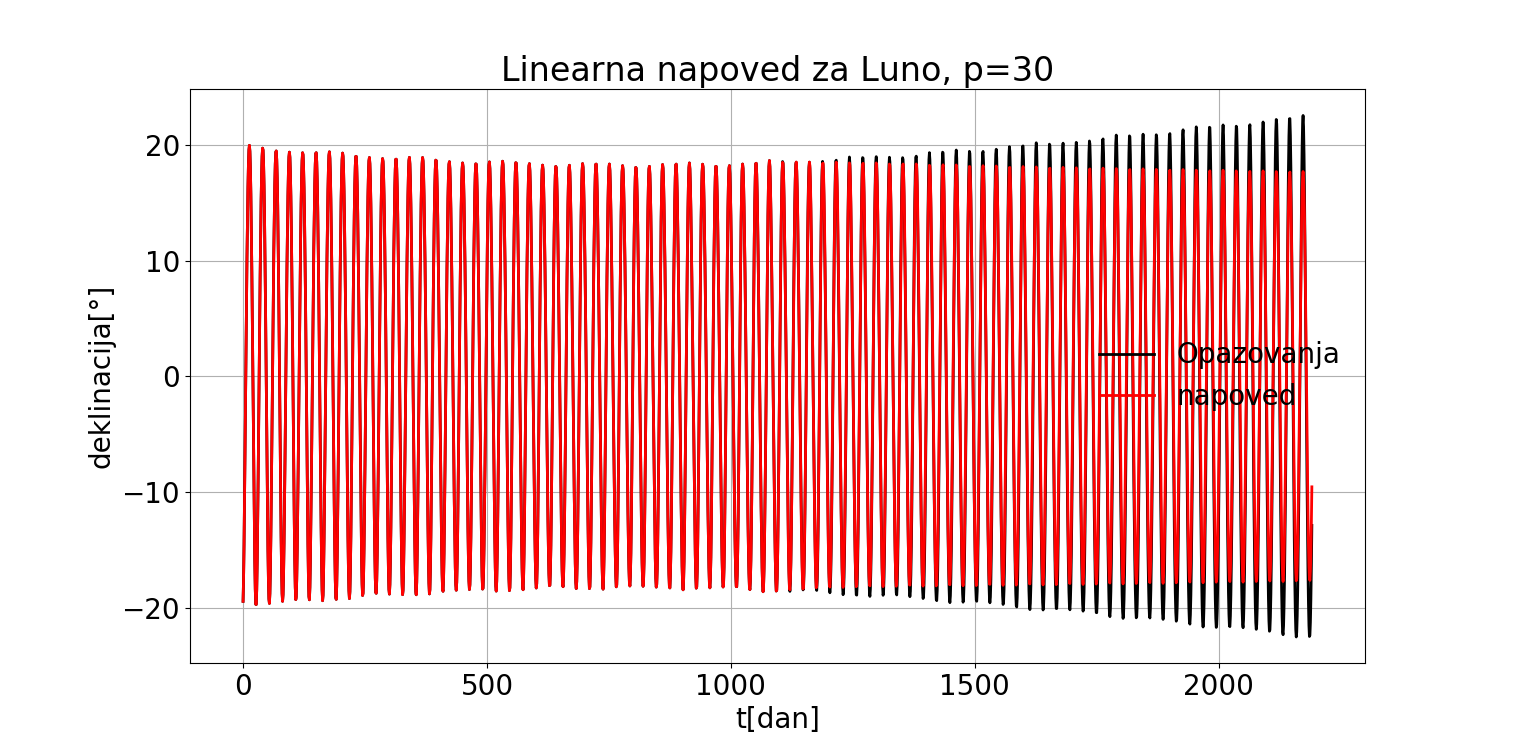
\includegraphics[width=8cm,height=5cm]{2.png}

\end{figure}
Vidimo da že za malo polov (10) popolnoma zadanemo frekvenco položaja lune, za boljšo amplitudo pa moramo vzeti več polov.
\subsection{Vpliv šuma na linearno napoved}
Vpliv šuma smo testirali tako da smo vzeli podatke iz signala $val2.dat$ in vsaki točki primešali beli šum naključno generirali iz normalne porazdelitve $N(0, \sigma)$, kjer smo spremnijali parameter $\sigma $ in tako vplivali na velikost šuma. Najprej si pogljemo napoved brez šuma. 
\begin{figure}[H]
\centering
  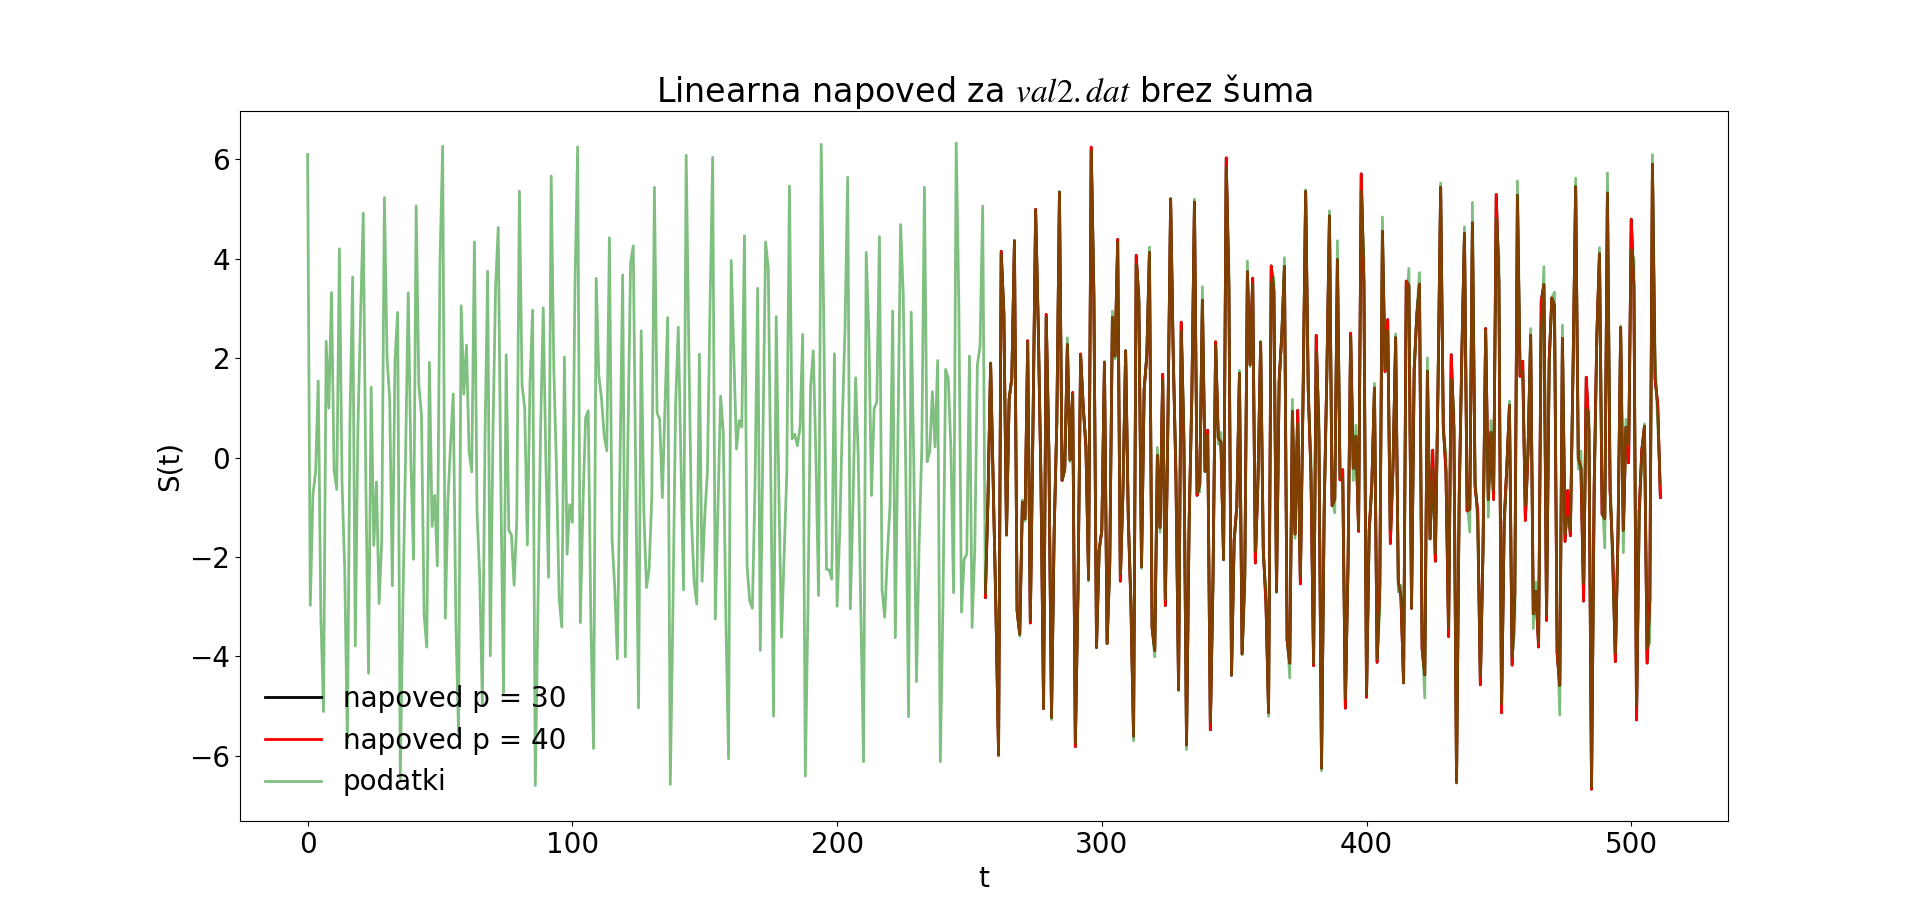
\includegraphics[width=16cm,height=5cm]{zadnja0.png}
 

\end{figure}
Za oba $p = 20,30$ je prileganje zelo dobro. Sedaj primešajmo šum in zopet izvedemo MEM.
\begin{figure}[H]
\centering

    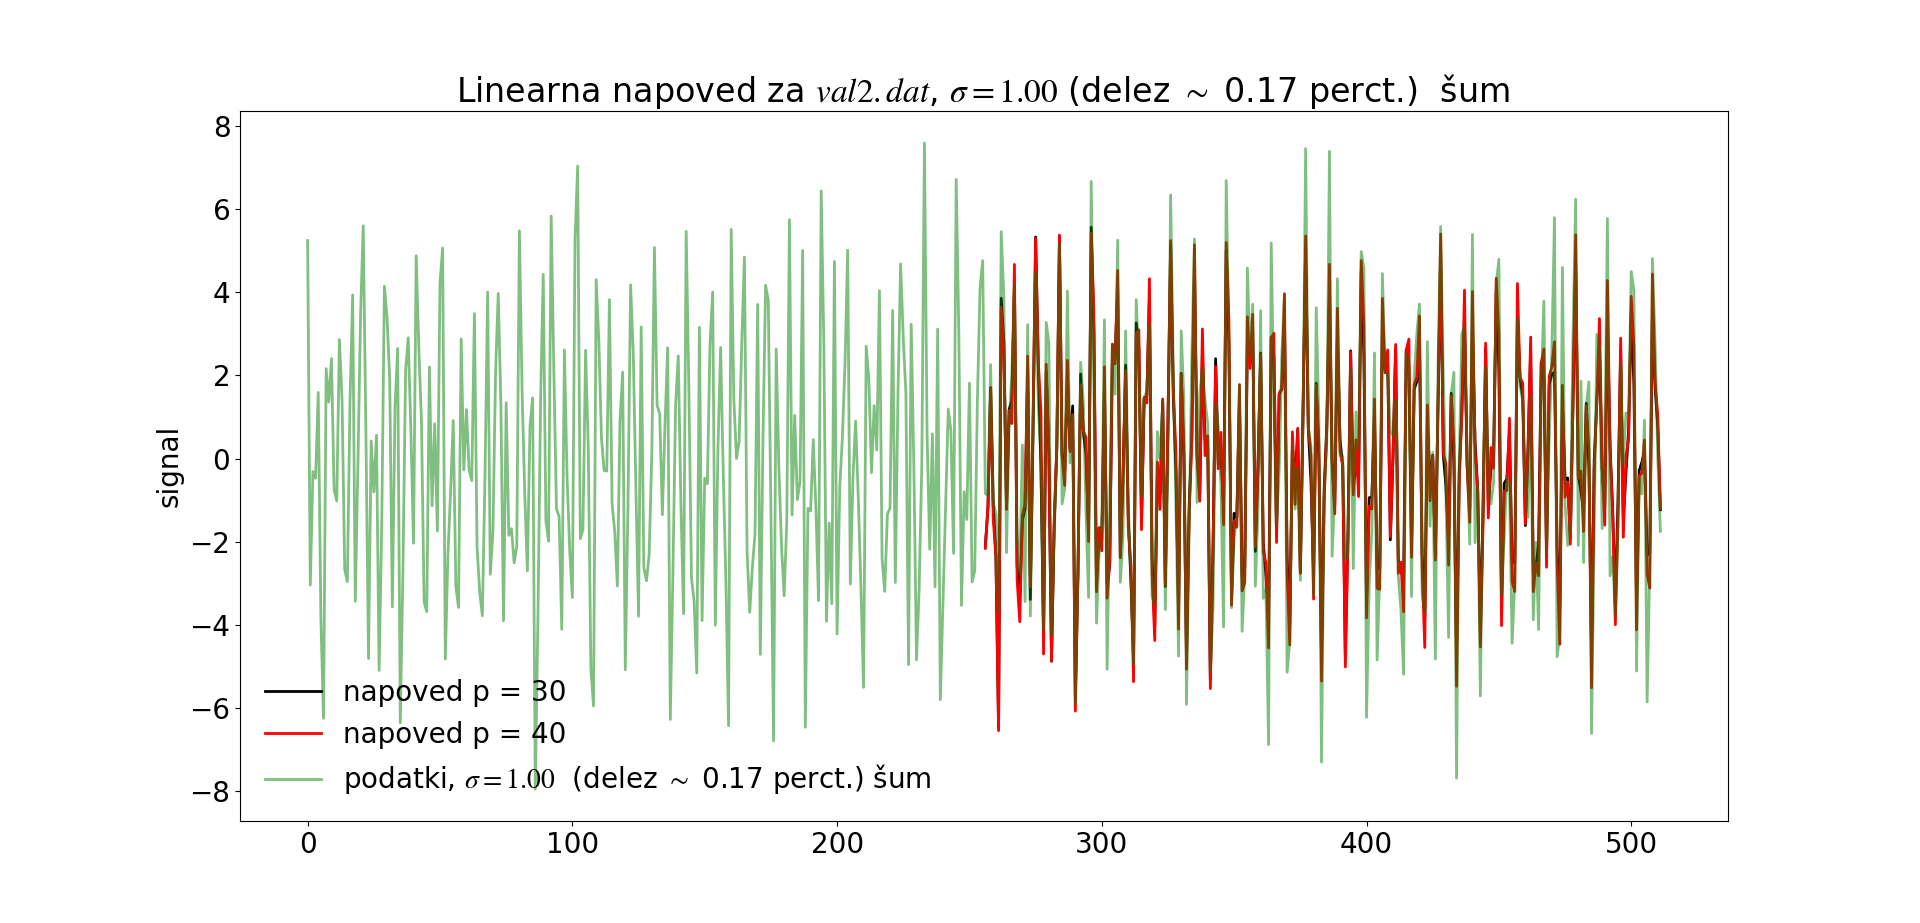
\includegraphics[width=16cm,height=5cm]{zadnja1.png}
 
   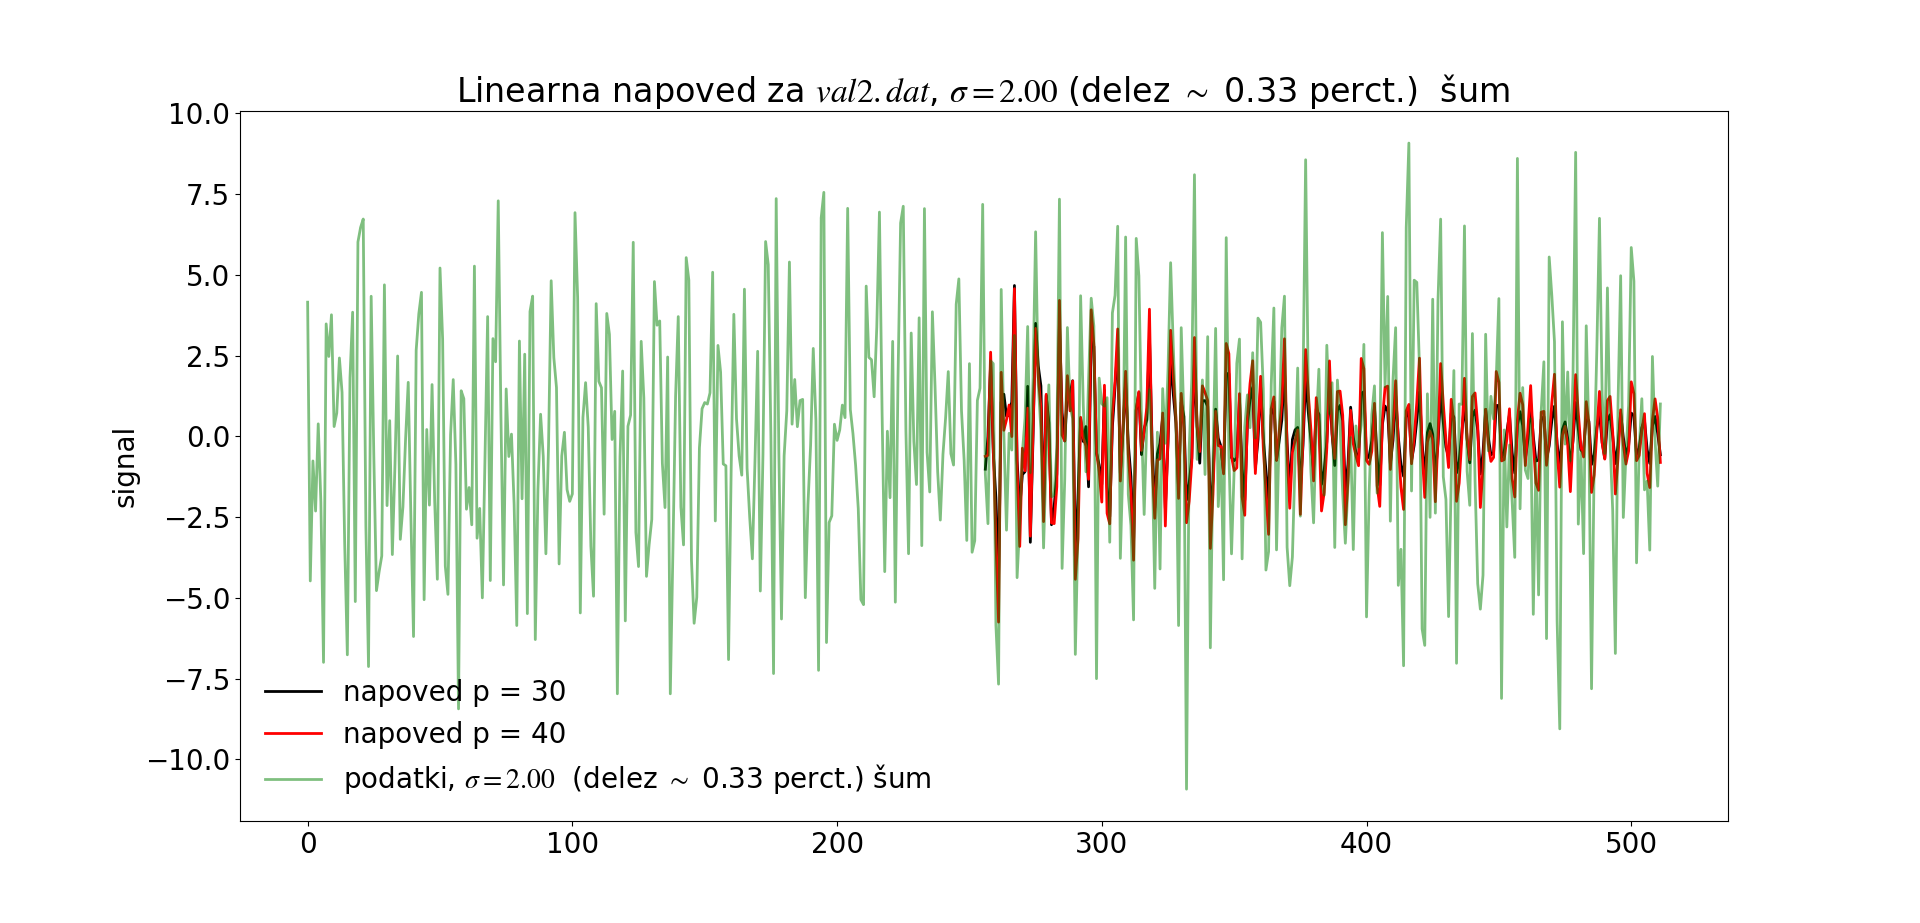
\includegraphics[width=16cm,height=5cm]{zadnja2.png}
    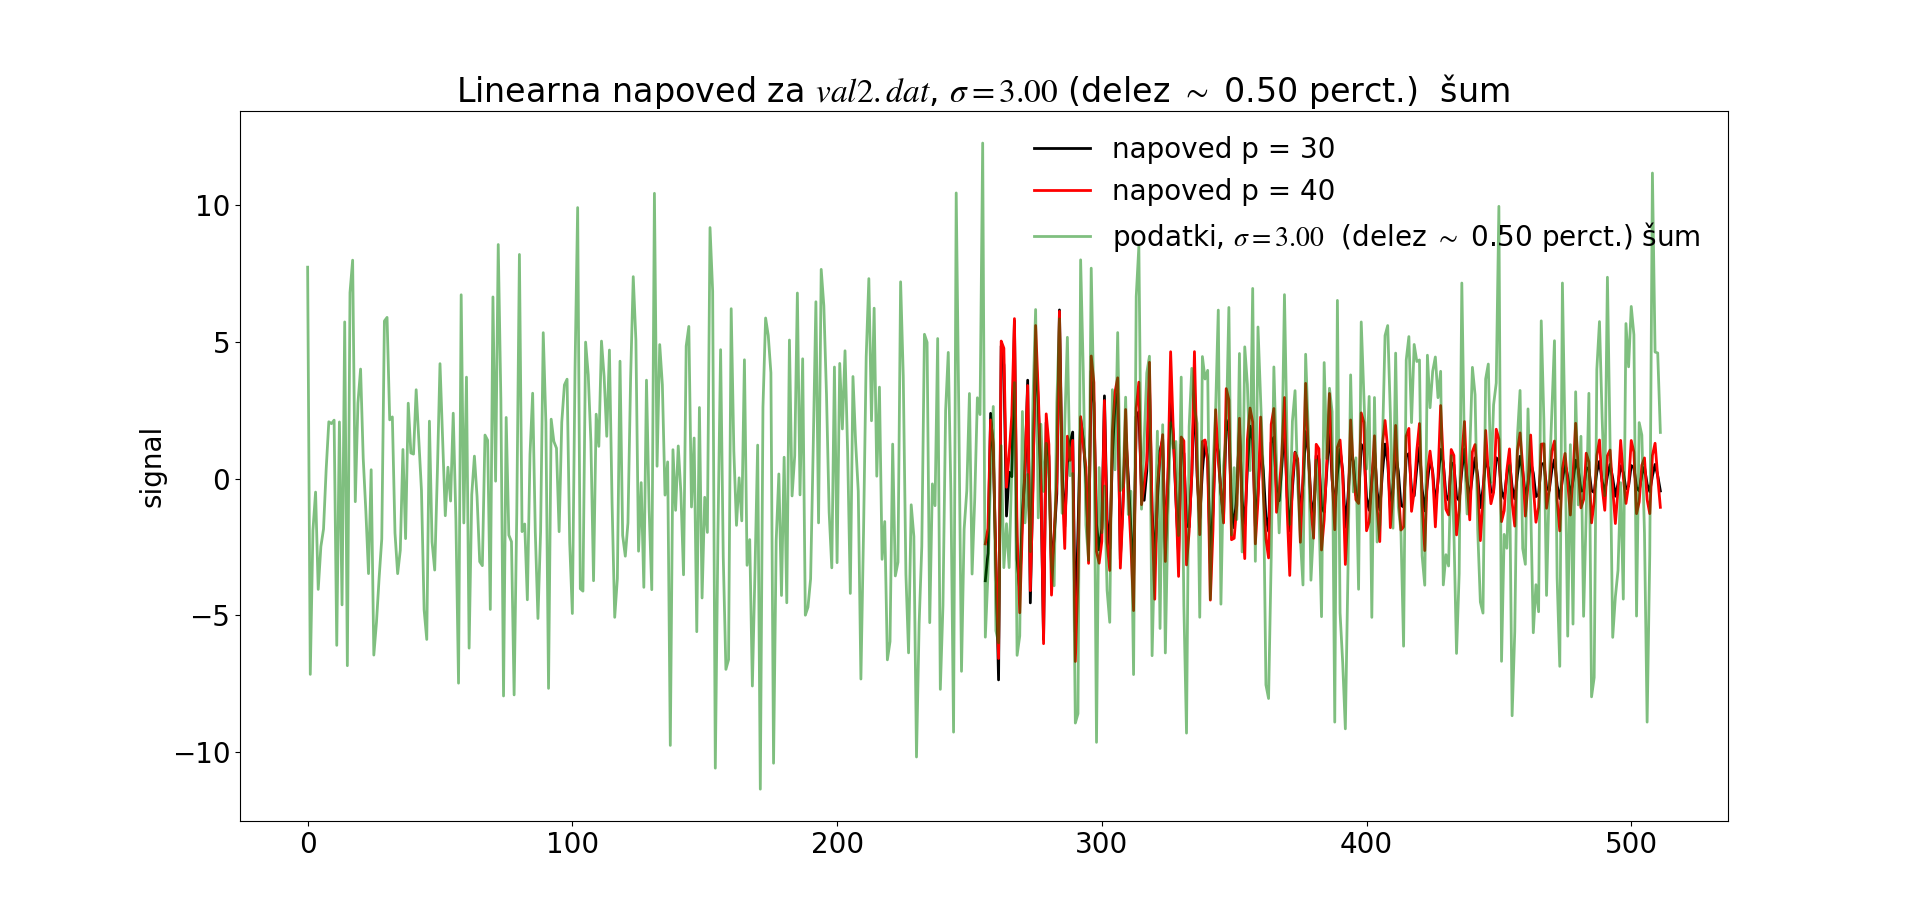
\includegraphics[width=16cm,height=5cm]{zadnja3.png}
     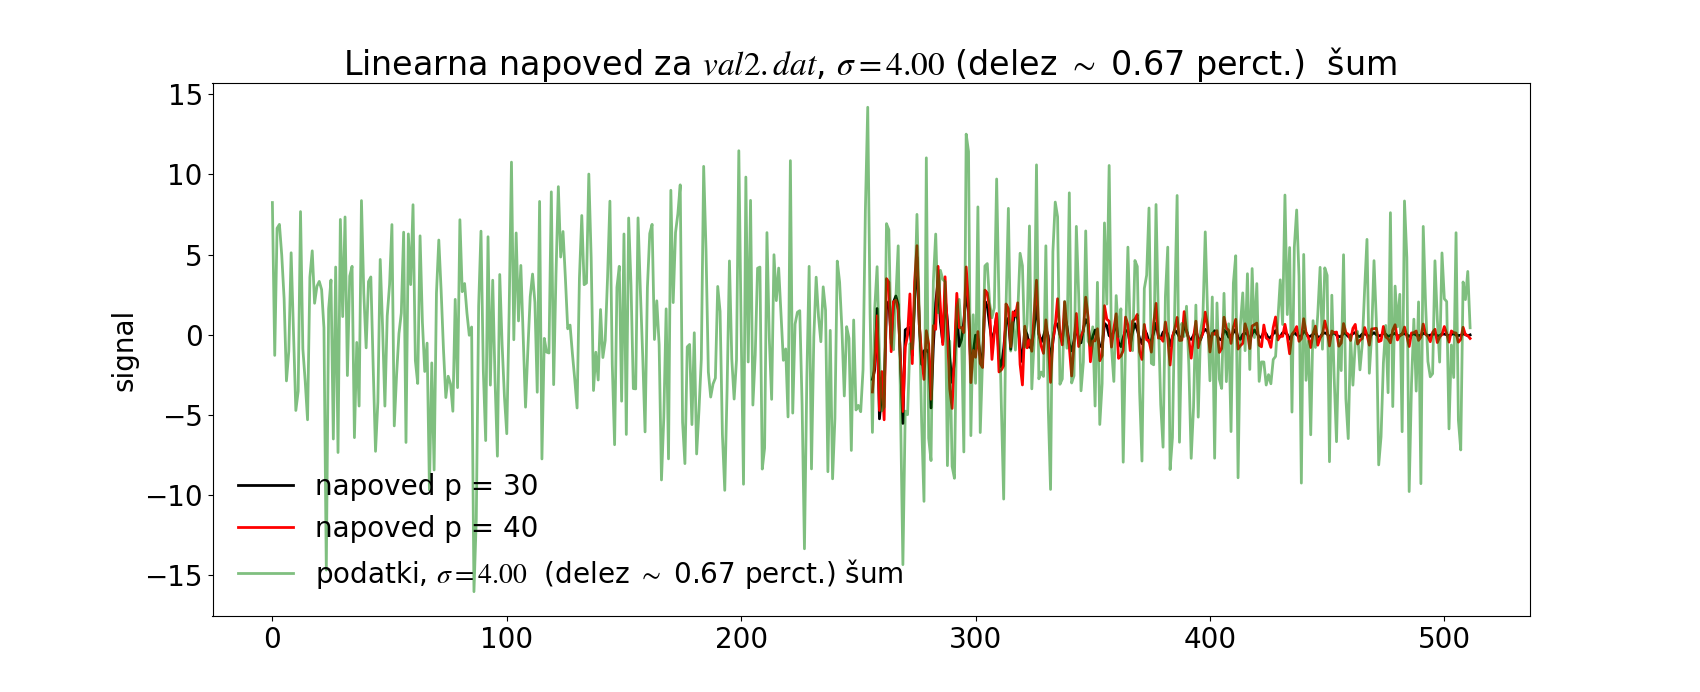
\includegraphics[width=16cm,height=5cm]{zadnja4.png}
 

\end{figure}
Vidimo da naša linearna napoved vse manj ustreza meritvam. Pri majhnem šumu napoved zgreši le amplitude, toda pri velikem šumu imamo problem tudi s frekvencami .Zavedati se moramo tudi da naša nova napoved želi napovedati zašumljene  podatke. Zanimivo se mi zdi da napovedan siganl za $p=40$ precej dobro ustreza amplitudam pravega signala.   \newline
Poglejmo si ali lahko signal popravimo če vzamemo več polov. Pogledali si bomo na primeru $\sigma = 3$
\begin{figure}[H]
\centering

    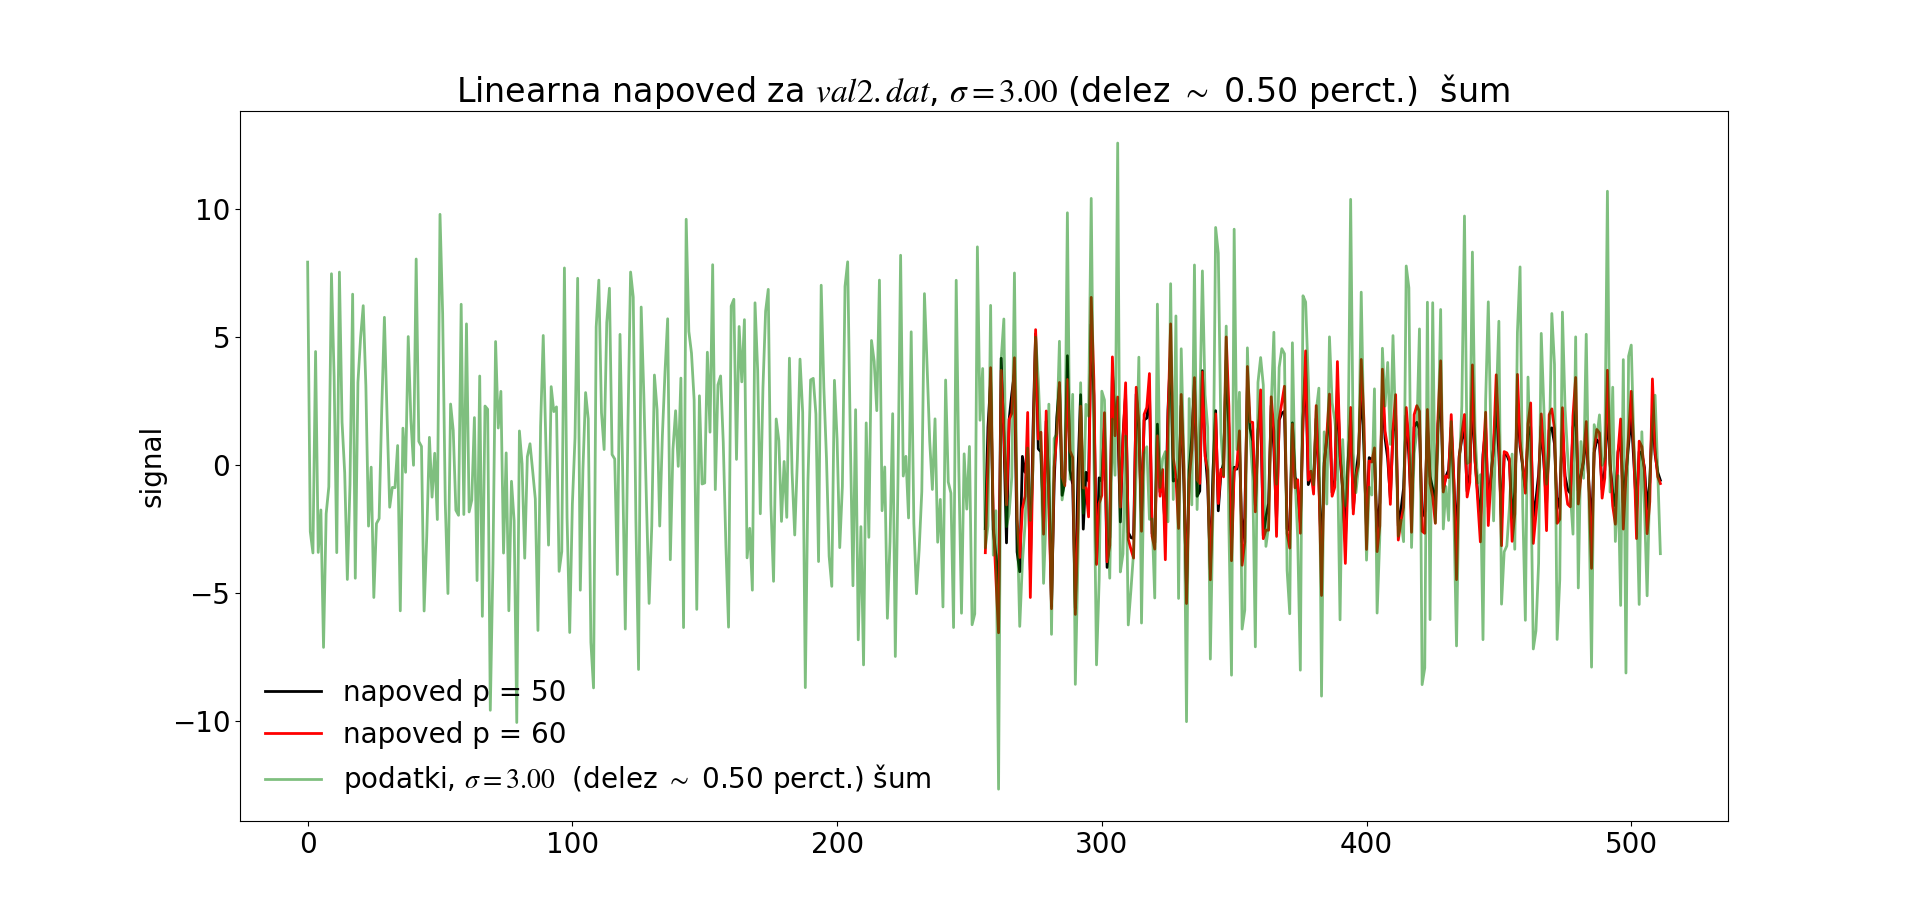
\includegraphics[width=16cm,height=7cm]{zadnja6.png}
   

\end{figure}
Pri zvišanju števila polov  $p=60$, močno popravimo napoved, čeprav imamo reda $\sim 50\%$ zašumljen signal. Pri večih polih linearna napoved zopet zdivergira.
\begin{figure}[H]
\centering

    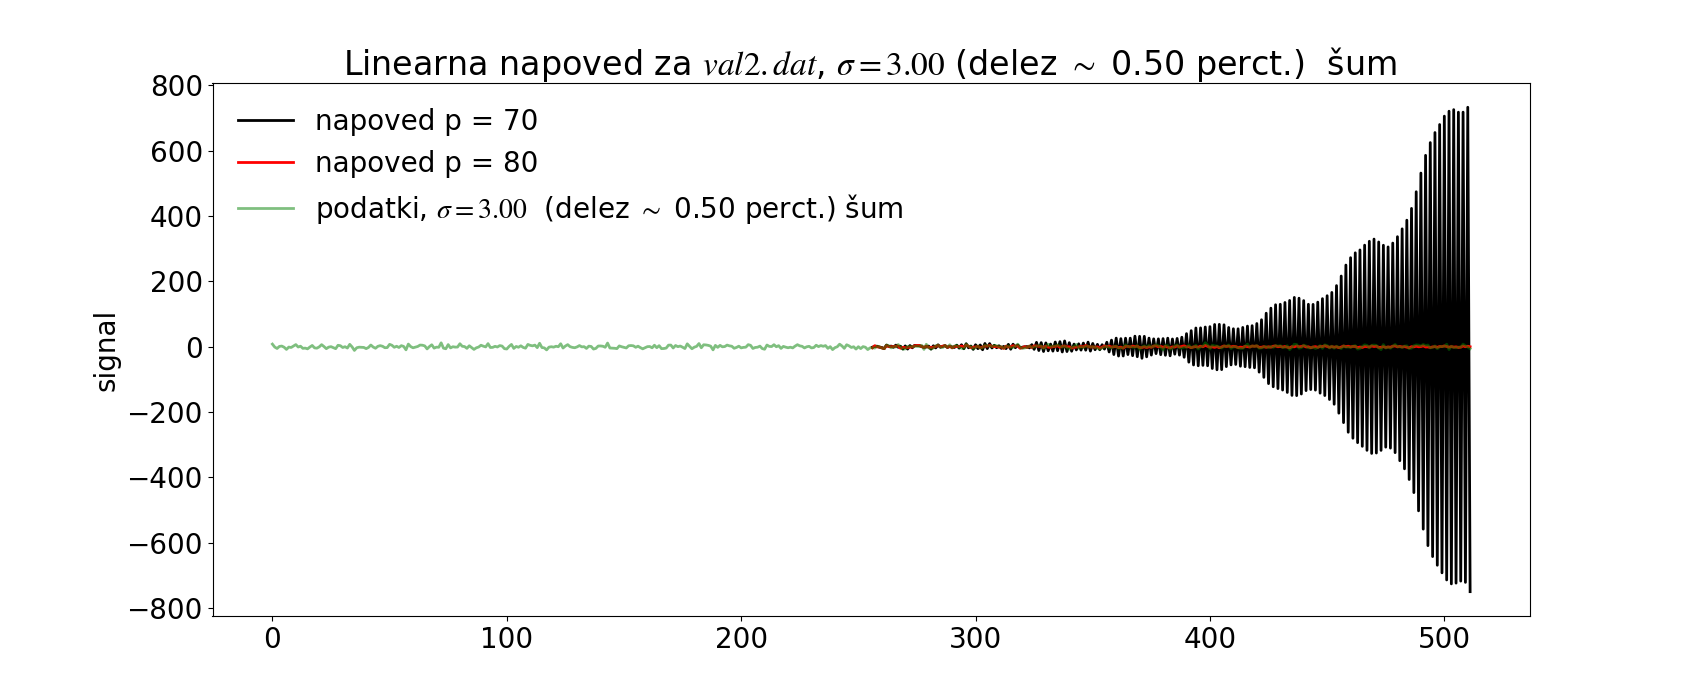
\includegraphics[width=16cm,height=7cm]{divergira2.png}
   

\end{figure}
\section{Zaključek}
Ogledali smo si delovanje, prednosti in slabosti metode MEM za spektre in linearno napovedovanje. Preučili smo ločljivost metode, vpliv šuma na napovedovanje in preiskusili MEM na različnih signalih. Ugotovili smo da bolj kot je preprost signal lažje ga je napovedovati, zato tudi na borzi napovedovanje žal ne deluje na tak način in potrebujemo močnejša orodja.

\end{document}